\documentclass{article}
\usepackage[utf8]{inputenc}
\usepackage[spanish]{babel}
\usepackage{array}
\usepackage{graphicx}
\usepackage{verbatim}
\usepackage{xcolor}
\definecolor{LightGray}{gray}{0.9}
\definecolor{White}{gray}{1.0}
\usepackage{tikz}
\usepackage{tabulary}
\usepackage{tabularx}
\usepackage{colortbl}
 \usepackage{booktabs} 
  \usepackage{multirow}
\usepackage{eurosym}
\usepackage[utf8]{inputenc}
\usepackage{amsmath}
\usepackage{amsmath}
\usepackage{amssymb}
\usepackage{vmargin}
\usepackage{multicol}
\setpapersize{A4}
\setmargins{2.5cm}       % margen izquierdo
{1.5cm}                        % margen superior
{16.5cm}                      % anchura del texto
{23.42cm}                    % altura del texto
{10pt}                           % altura de los encabezados
{1cm}                           % espacio entre el texto y los encabezados
{0pt}                             % altura del pie de página
{2cm}                           % espacio entre el texto y el pie de página

\usepackage{multicol,caption}
\newenvironment{Figure}
  {\par\medskip\noindent\minipage{\linewidth}}
  {\endminipage\par\medskip}
  
\usepackage{hyperref}
\hypersetup{
    colorlinks=true,
    linkcolor=black,
    filecolor=magenta,      
    urlcolor=cyan,
    citecolor = black,
    pdfpagemode=FullScreen,
    }
\usepackage{minted}
\begin{document}
\begin{titlepage}

    \begin{tikzpicture}[remember picture,overlay]
    \node[anchor=north west,yshift=50pt,xshift=0.7\textwidth]%
        at (current page.north west)
        {
\includegraphics[width=0.2\textwidth]{Imágenes/logo.png}};
    \end{tikzpicture}

\centering
\vspace{4cm}
{\bfseries\LARGE Universidad de Córdoba\par}
\vspace{0.5cm}
{\scshape\Large Máster en Inteligencia Computacional e Internet de las Cosas \par}
\vspace{3cm}
{\scshape\Huge Memoria de Prácticas \par}
\vspace{1cm}
{\scshape\Large  \par}
\vspace{1.5cm}
{\itshape\Large  \par}
\vfill
{\Large Autor: Alberto Fernández Merchán \par}
{\Large Asignatura: Análisis Automático de Datos para las Ciencias Biomédicas, Medioambientales,
Agroalimentarias. \par}
\vfill
{\Large Profesor: Javier Sánchez Monedero \par}
{\Large Junio 2025}
{\Large  \par}
\end{titlepage}
\newpage

\tableofcontents
\listoftables


\newpage

\section{Introducción}

El análisis de datos y la construcción de modelos predictivos se han convertido en una parte fundamental del aprendizaje automático y la ciencia de datos. Para facilitar estas tareas, existen diversas herramientas que permiten a los usuarios aplicar técnicas de preprocesamiento, selección de características, entrenamiento y evaluación de modelos sin necesidad de programación avanzada. Entre ellas, destaca \textbf{WEKA} (Waikato Environment for Knowledge Analysis) \cite{weka2016}, una plataforma de software libre desarrollada por la Universidad de Waikato, ampliamente utilizada en la comunidad académica para el análisis y minería de datos.\\

Este trabajo tiene como objetivo explorar el ciclo completo de desarrollo de un modelo predictivo utilizando WEKA, desde la preparación de los datos hasta la evaluación de su rendimiento. A lo largo del documento se aplican distintas técnicas sobre dos conjuntos de datos: \texttt{Audiology\_soft} y \texttt{Glass Identification}. El primero se emplea para ilustrar las fases de preprocesamiento, mientras que el segundo se utiliza como caso práctico para construir y evaluar modelos de clasificación. \\

En primer lugar, se abordan tareas esenciales de limpieza y transformación de datos, como la eliminación e imputación de valores perdidos, así como la conversión de atributos nominales a binarios. Posteriormente, se analiza un caso práctico donde se exploran las variables del conjunto de datos, su correlación y su distribución, permitiendo comprender mejor las características que pueden influir en la predicción.\\

A continuación, se estudia el efecto de la normalización y estandarización de los atributos sobre el rendimiento de varios algoritmos de clasificación implementados en WEKA, incluyendo \texttt{SimpleLogistic}, \texttt{J48} y \texttt{RandomForest}. Para cada caso, se presentan los resultados de entrenamiento y prueba utilizando validación cruzada, y se comparan los clasificadores a través de métricas como la precisión, el coeficiente de Kappa, el MAE, el RMSE, el F1-score, el coeficiente de correlación de Matthews (MCC) y el área bajo la curva ROC (AUC).\\

Finalmente, se extraen conclusiones sobre el comportamiento de los clasificadores ante diferentes preprocesamientos y se discuten las ventajas y limitaciones del uso de WEKA como entorno de análisis de datos.\\

\section{Preprocesado de Audiology\_soft}

En este apartado se detalla el proceso de preprocesado aplicado al conjunto de datos \textit{Audiology\_soft}, que trata sobre la clasificación de enfermedades auditivas a partir de diversos atributos clínicos. El conjunto original contiene 226 instancias y 10 atributos, además de la clase objetivo (\textit{class}), como se muestra en la Figura~\ref{fig:audiology-soft} y la Figura~\ref{fig:attributes-audiology}.

\begin{figure}[!ht]
    \centering
    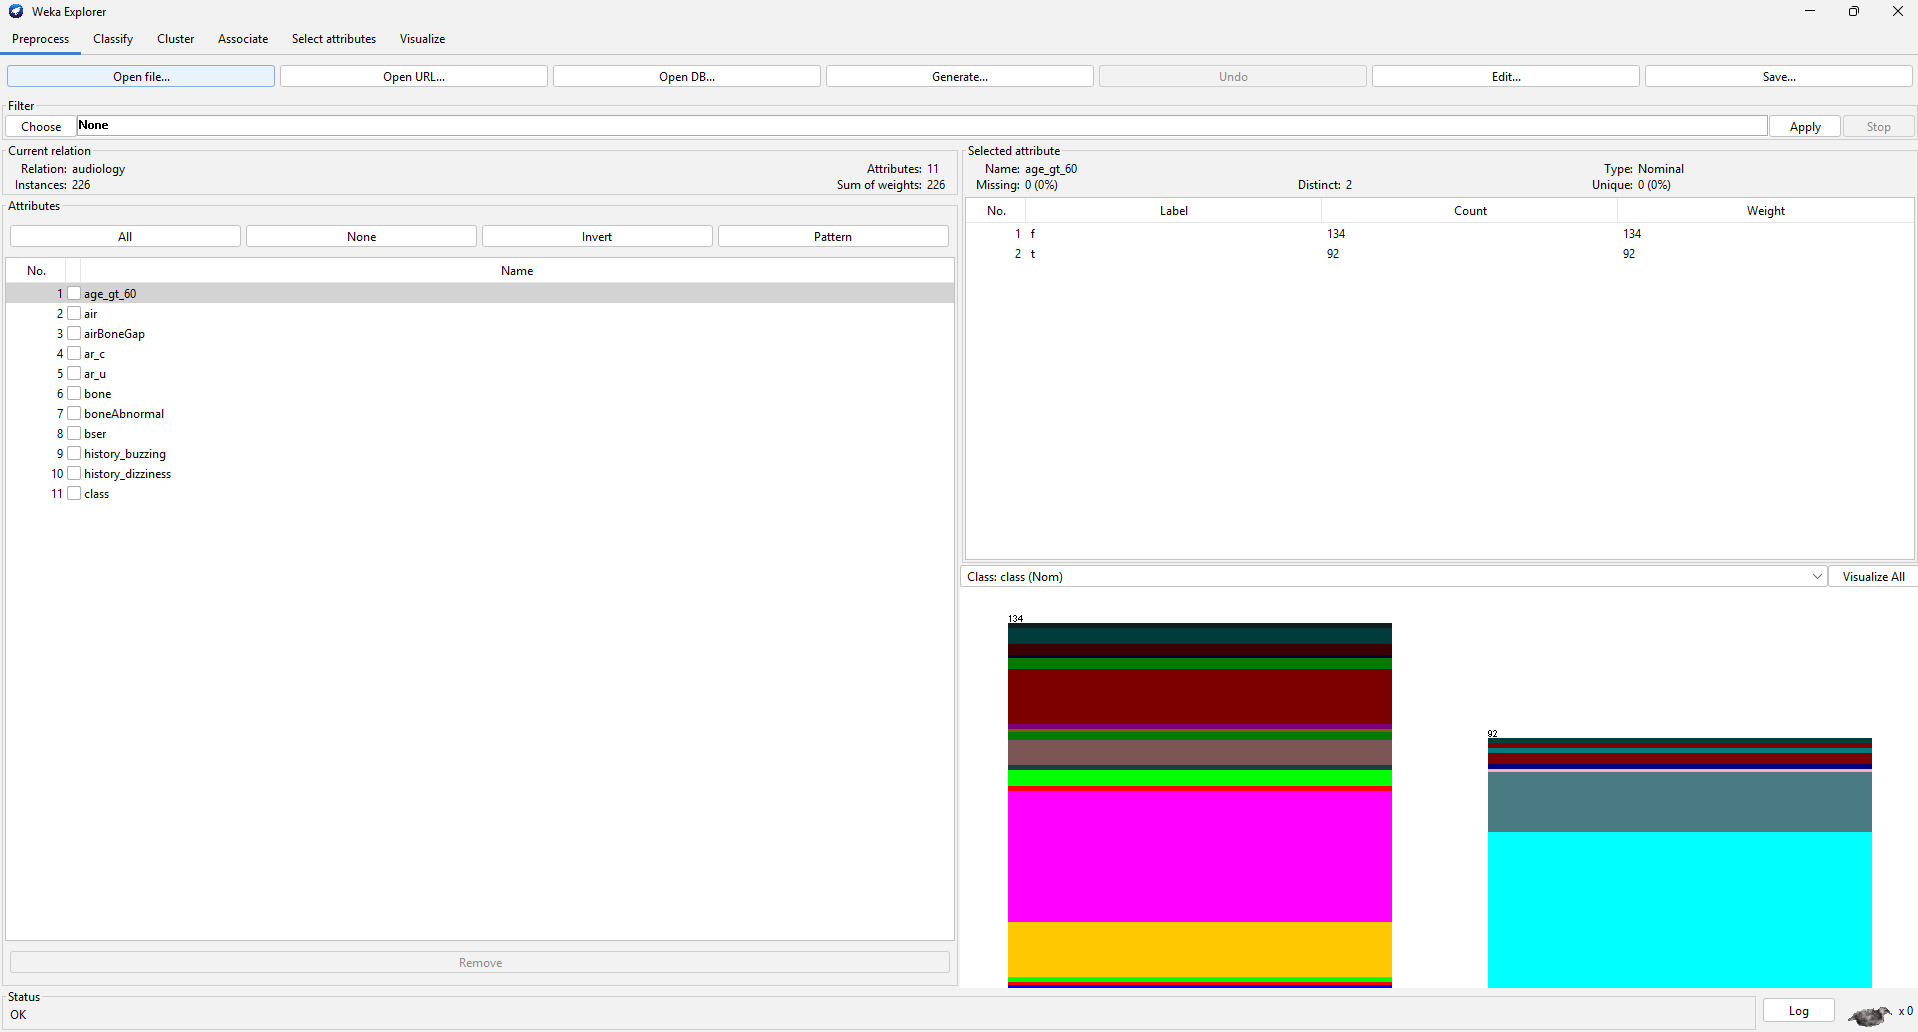
\includegraphics[width=0.9\linewidth]{Imágenes/audiology_init.png}
    \caption{Pantalla de visualización de datos en Weka del dataset de Audiology\_soft.}
    \label{fig:audiology-soft}
\end{figure}

\begin{figure}[!ht]
    \centering
    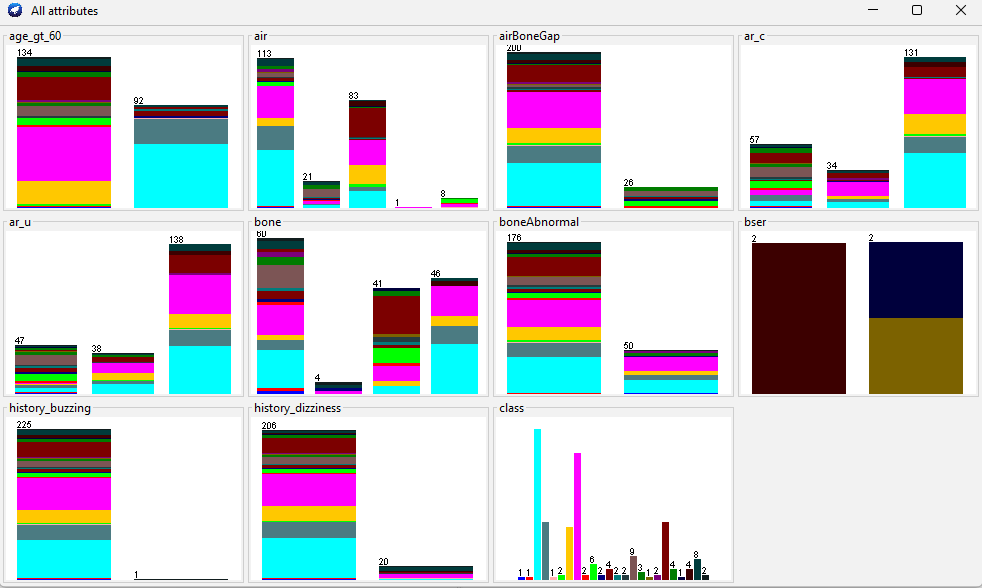
\includegraphics[width=0.9\linewidth]{Imágenes/atributos_dataset_audiology.png}
    \caption{Distribución de los valores de los atributos del dataset.}
    \label{fig:attributes-audiology}
\end{figure}

\newpage
\subsection{Eliminación de atributos con demasiados valores perdidos}

Se ha analizado el porcentaje de valores faltantes por cada atributo para determinar si eran susceptibles de imputación mediante la media o la moda. Se consideró que atributos con más de un 30\% de valores perdidos podrían introducir sesgos si se imputaban, por lo que estos fueron eliminados. 

El atributo \textit{bser} fue eliminado inmediatamente debido a que presentaba un 98\% de valores perdidos (Figura~\ref{fig:bser}).

\begin{figure}[!ht]
    \centering
    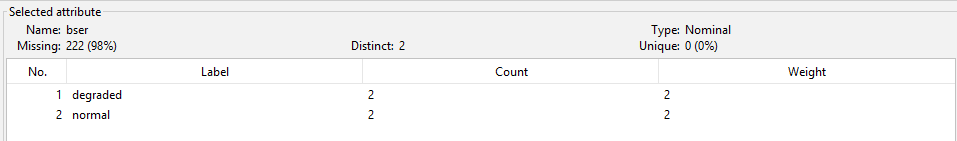
\includegraphics[width=1\linewidth]{Imágenes/attribute_bser.png}
    \caption{Información sobre el atributo \textit{bser} con un 98\% de valores perdidos.}
    \label{fig:bser}
\end{figure}

El atributo \textit{bone} tenía un 33\% de valores faltantes (Figura~\ref{fig:bone-delete}), por lo que inicialmente se valoró su eliminación por simplicidad. Sin embargo, en un análisis de selección de atributos, se observó que \textit{bone} tenía cierto valor predictivo (Figura~\ref{fig:bone-subset}).

\begin{figure}[!ht]
    \centering
    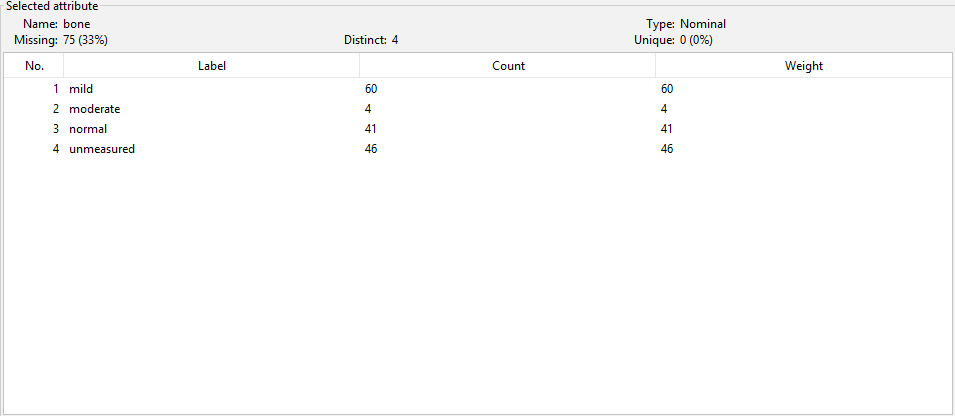
\includegraphics[width=\linewidth]{Imágenes/bone-attribute.png}
    \caption{Información sobre el atributo \textit{bone} con un 33\% de valores perdidos.}
    \label{fig:bone-delete}
\end{figure}

\begin{figure}[!ht]
    \centering
    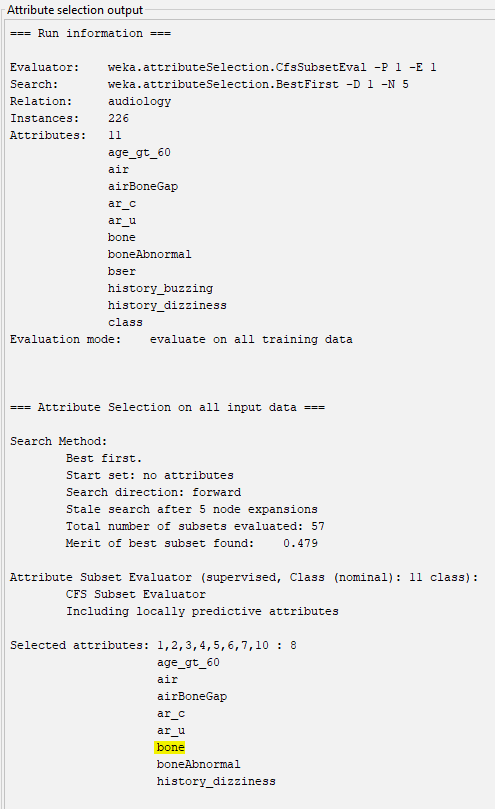
\includegraphics[width=0.8\linewidth]{Imágenes/bone-attribute-search.png}
    \caption{En la selección de atributos nos aparece que el atributo \textit{bone} tiene valor predictivo.}
    \label{fig:bone-subset}
\end{figure}

\newpage
Pese a ello, al repetir el proceso de selección sin dicho atributo, el mérito del subconjunto seleccionado fue idéntico (0.479), como se puede observar en la Figura~\ref{fig:attribute-without-bone}, por lo que finalmente se decidió eliminar también el atributo \textit{bone} para simplificar el conjunto.

\begin{figure}[!ht]
    \centering
    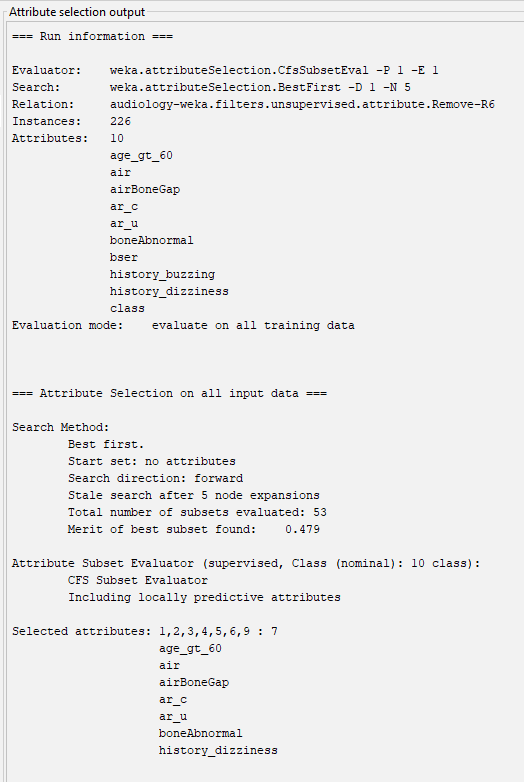
\includegraphics[width=0.8\linewidth]{Imágenes/reduced-attribute-search.png}
    \caption{Selección de atributos sin incluir \textit{bone}; el mérito del subconjunto permanece igual.}
    \label{fig:attribute-without-bone}
\end{figure}

El dataset resultante queda reducido a 8 atributos más la clase (Figura~\ref{fig:final-dataset}).

\begin{figure}[!ht]
    \centering
    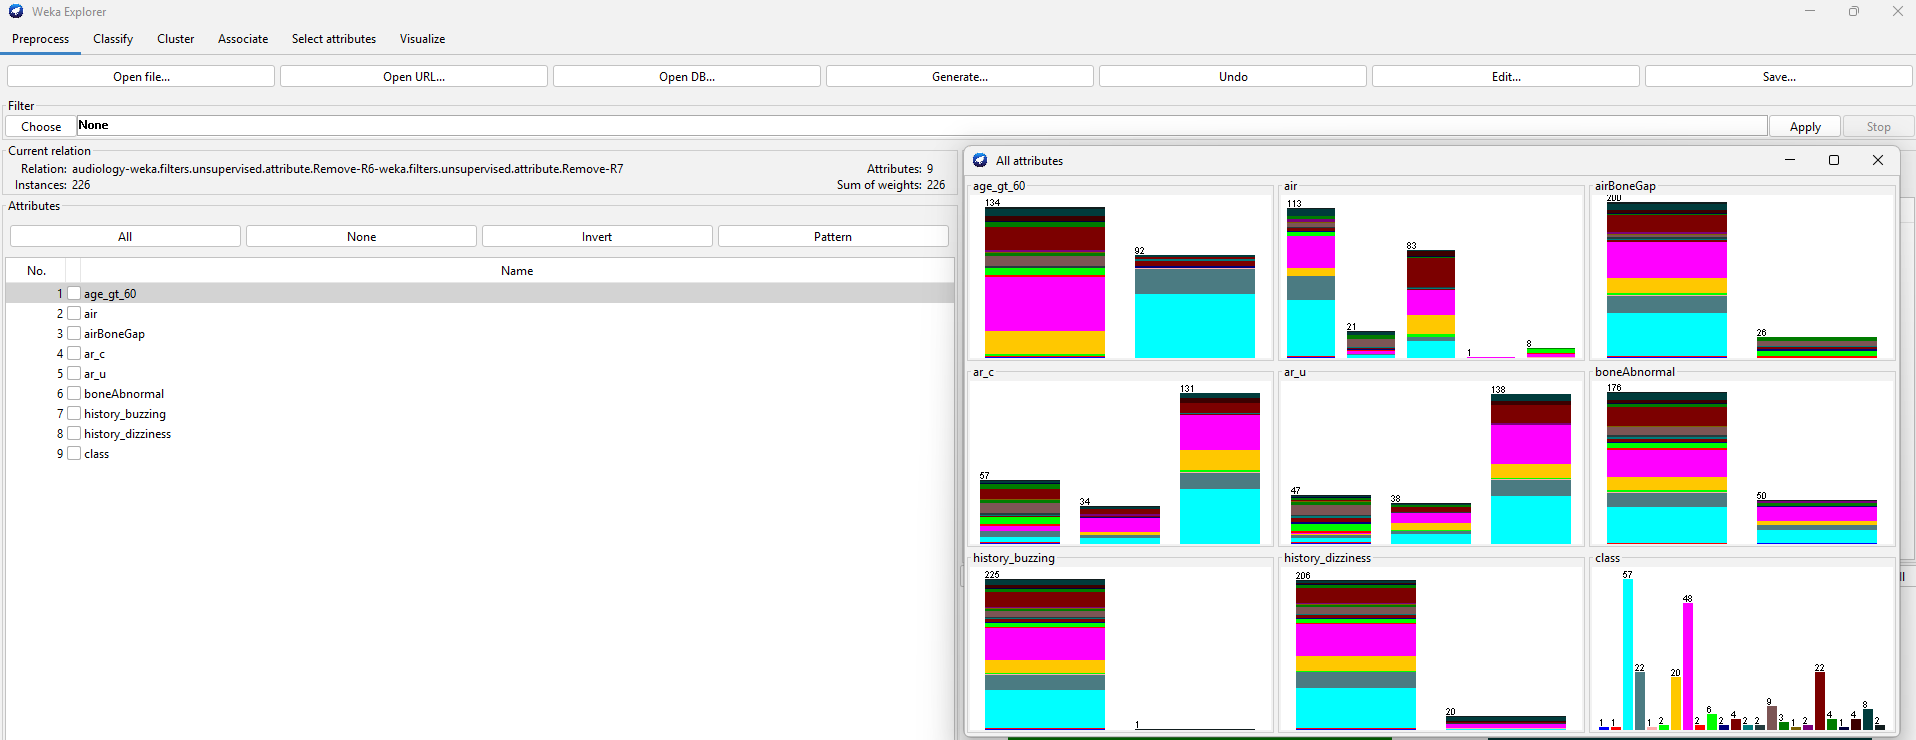
\includegraphics[width=1\linewidth]{Imágenes/final_dataset.png}
    \caption{Conjunto de datos final con los atributos eliminados.}
    \label{fig:final-dataset}
\end{figure}

\subsection{Imputación de valores perdidos}

A continuación, se aplicó el filtro \texttt{ReplaceMissingValues}, que imputa automáticamente los valores faltantes restantes. Para atributos nominales, emplea la moda; para atributos numéricos, la media. Tras aplicar este filtro, se verificó que no quedaban valores faltantes, ya que la suma de valores por atributo coincide con el número total de instancias (Figura~\ref{fig:no-missing}).

\begin{figure}[!ht]
    \centering
    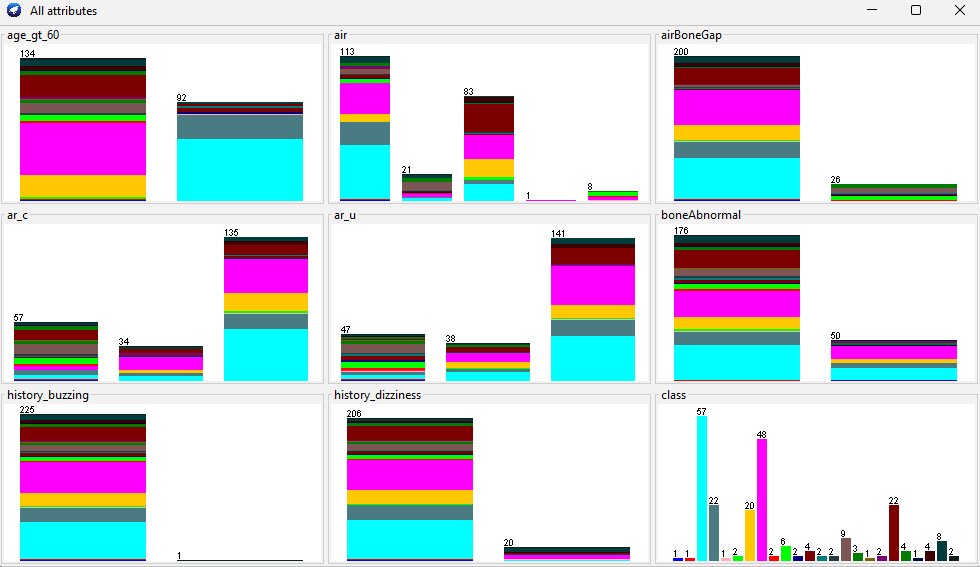
\includegraphics[width=1\linewidth]{Imágenes/no-missing-values.png}
    \caption{Conjunto de datos sin valores perdidos (todos los atributos suman 226, el número de instancias del dataset).}
    \label{fig:no-missing}
\end{figure}

\subsection{Conversión de atributos nominales a binarios}

Finalmente, se aplicó el filtro \texttt{NominalToBinary} sobre los atributos nominales binarios y categórico como se muestra en la Figura~\ref{fig:binary_attr}. 

\begin{figure}[!ht]
    \centering
    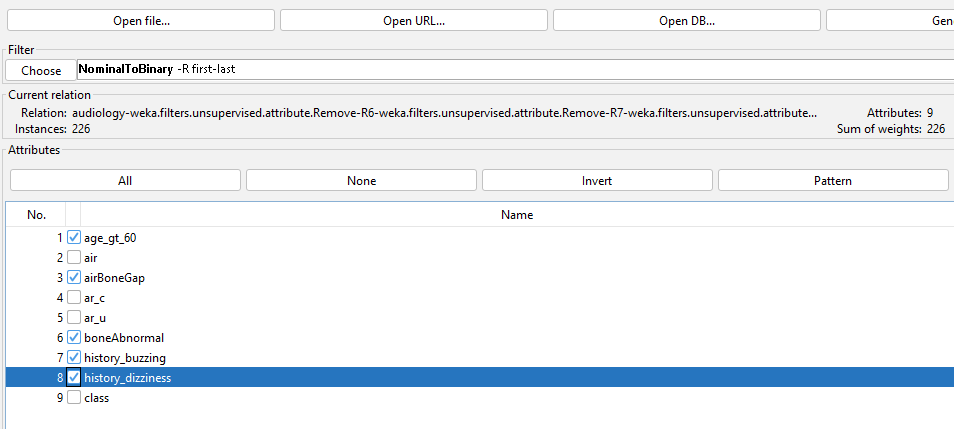
\includegraphics[width=1\linewidth]{Imágenes/valores_binarios.png}
    \caption{Selección de atributos con valores binarios del conjunto de datos.}
    \label{fig:binary_attr}
\end{figure}

Al aplicar el filtro, cada atributo nominal seleccionado fue transformado en una o más variables binarias, permitiendo representar la información de forma numérica (Figura~\ref{fig:nominal-to-binary}).

\begin{figure}[!ht]
    \centering
    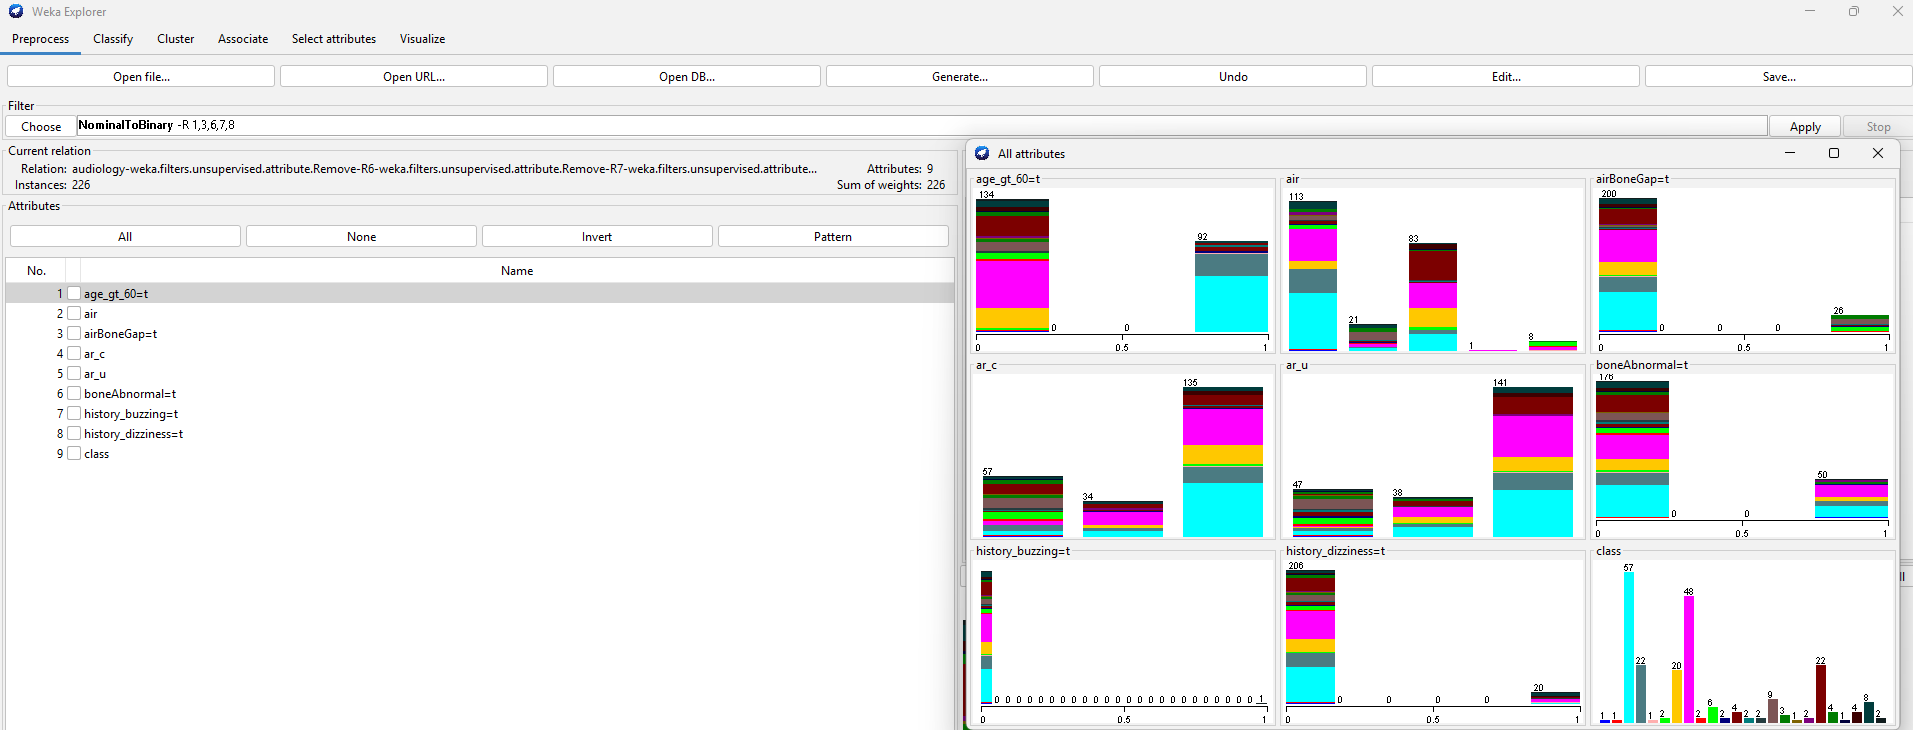
\includegraphics[width=1\linewidth]{Imágenes/NominalToBinary.png}
    \caption{Conjunto de datos tras aplicar el filtro \texttt{NominalToBinary} a los atributos binarios (1, 3, 6, 7, 8).}
    \label{fig:nominal-to-binary}
\end{figure}

\newpage

\section{Elección de Caso Práctico}

% % Se ha elegido el dataset de Glass:
%  Glass Identification. Base de datos del Servicio de Ciencias Forenses de EE.UU. donde se
% identifican 6 tipos de vidrio en función de su contenido en óxidos. En esta base de datos debes
% eliminar la variable del identificador de la muestra. (https://archive.ics.uci.edu/dataset/42/glass+identification)

El conjunto de datos seleccionado para el desarrollo del caso práctico es \textit{Glass Identification}, disponible en el repositorio de aprendizaje automático de la Universidad de California en Irvine (UCI)~\footnote{\url{https://archive.ics.uci.edu/dataset/42/glass+identification}}. Esta base de datos, proporcionada por el Servicio de Ciencias Forenses de los Estados Unidos, tiene como propósito la clasificación de distintos tipos de vidrio a partir de su composición química.\\

El objetivo principal consiste en determinar a qué tipo pertenece una muestra de vidrio, utilizando como base el porcentaje de diversos óxidos presentes en su estructura. Las clases recogidas en el conjunto de datos incluyen vidrios de ventanas (flotadas y no flotadas), vidrios de automóviles, utensilios, contenedores, entre otros.\\

El dataset está compuesto por 214 instancias y 10 atributos. Entre los atributos se encuentran las concentraciones de los siguientes compuestos: óxido de sodio (\texttt{Na}), óxido de magnesio (\texttt{Mg}), óxido de aluminio (\texttt{Al}), óxido de silicio (\texttt{Si}), óxido de potasio (\texttt{K}), óxido de calcio (\texttt{Ca}), óxido de bario (\texttt{Ba}) y óxido de hierro (\texttt{Fe}). Además, se incluye el índice de refracción (\texttt{RI}) y una variable identificadora que, por su naturaleza, no aporta valor predictivo.\\

La Figura~\ref{fig:dataset} muestra una vista inicial del dataset cargado en el entorno de trabajo.\\

\begin{figure}[!ht]
    \centering
    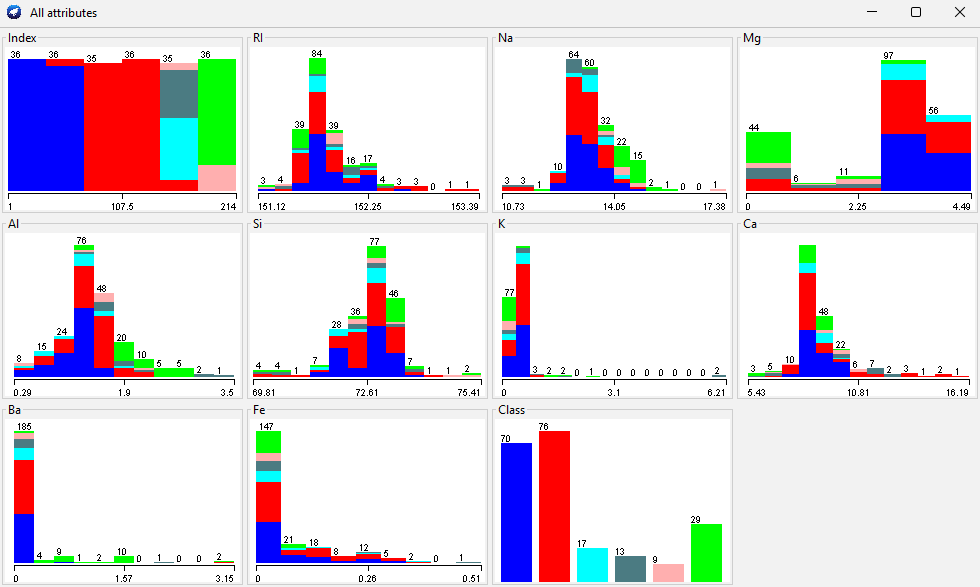
\includegraphics[width=1\linewidth]{Imágenes/dataset-glass.png}
    \caption{Vista inicial del dataset \textit{Glass Identification} en Weka.}
    \label{fig:dataset}
\end{figure}

Dado que el identificador de la muestra no contiene información útil para el proceso de clasificación y puede introducir ruido en los modelos, se ha optado por eliminar esta variable durante la fase de preprocesamiento. El resto de atributos, todos de tipo numérico continuo, son aptos para ser utilizados en algoritmos estadísticos y de aprendizaje automático.\\

Una vez eliminado el identificador, el conjunto de datos queda como se observa en la Figura~\ref{fig:dataset-sin-id}.\\

\begin{figure}[!ht]
    \centering
    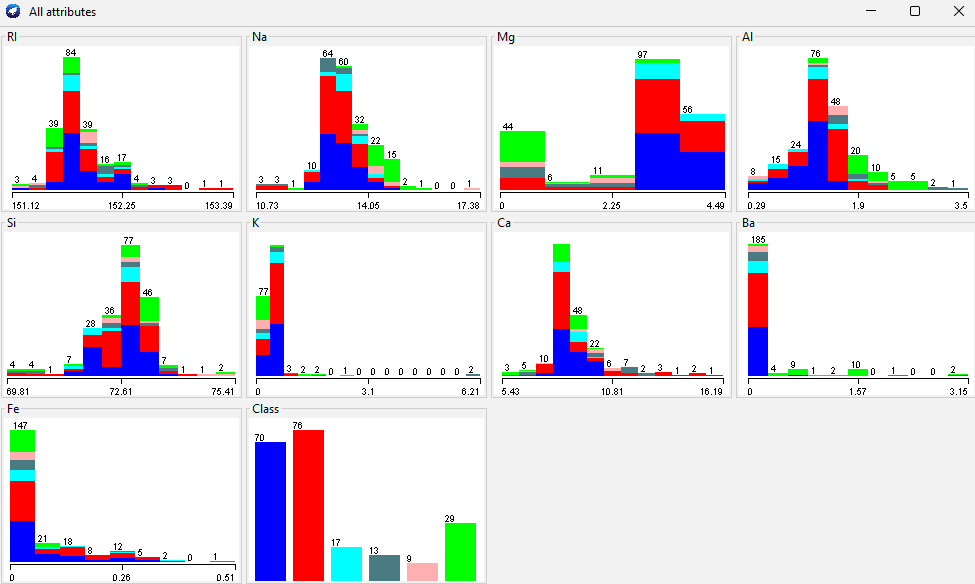
\includegraphics[width=1\linewidth]{Imágenes/dataset-sin-id.png}
    \caption{Vista del dataset tras eliminar la variable identificador.}
    \label{fig:dataset-sin-id}
\end{figure}

\section{Análisis Preliminar}\label{sec:seleccion-caracteristicas}
% Desde el entorno Preprocess, cargue la base de datos en Weka e indiqué que tipo de problema
% está estudiando. Por cada variable, comente su significado o de qué se trata y cuál es su tipo (el
% uso de tablas agilizará su interpretación y lectura). Puede hacer también comentarios sobre las
% variables que desee y que quiera destacar. Además de la información que aporta Weka, puede
% ayudarse de la información disponible en los ficheros .names y .txt, que está recogida del propio
% repositorio de la UCI:

Una vez cargado el dataset en el entorno \texttt{Preprocess} de Weka, se puede confirmar que se trata de un problema de clasificación multiclase, ya que la variable objetivo es de tipo categórico y toma uno de los siete posibles valores correspondientes a distintos tipos de vidrio. Todos los atributos predictivos son numéricos continuos, lo que permite aplicar algoritmos de análisis y clasificación.\\

La Tabla~\ref{tab:variables-glass} resume las características principales de cada variable del conjunto de datos, incluyendo su nombre, una breve descripción, el tipo de dato y observaciones adicionales de interés.\\

\begin{table}[H]
    \centering
    \caption{Descripción de las variables del dataset \textit{Glass Identification}.}
    \label{tab:variables-glass}
    \begin{tabular}{|c|p{6cm}|c|p{5cm}|}
        \hline
        \textbf{Nombre} & \textbf{Descripción} & \textbf{Tipo} & \textbf{Observaciones} \\
        \hline
        RI & Índice de refracción & Numérico & Medida óptica que varía ligeramente entre tipos de vidrio \\
        \hline
        Na & Porcentaje de óxido de sodio (\%) & Numérico & Elemento habitual en la mayoría de los vidrios \\
        \hline
        Mg & Porcentaje de óxido de magnesio (\%) & Numérico & Presente principalmente en vidrio de contenedores \\
        \hline
        Al & Porcentaje de óxido de aluminio (\%) & Numérico & Mejora la resistencia del vidrio \\
        \hline
        Si & Porcentaje de óxido de silicio (\%) & Numérico & Principal componente de la mayoría de los vidrios \\
        \hline
        K  & Porcentaje de óxido de potasio (\%) & Numérico & Presente en algunos tipos específicos de vidrio \\
        \hline
        Ca & Porcentaje de óxido de calcio (\%) & Numérico & Común en vidrios para ventanas y botellas \\
        \hline
        Ba & Porcentaje de óxido de bario (\%) & Numérico & Distintivo de algunos vidrios especiales \\
        \hline
        Fe & Porcentaje de óxido de hierro (\%) & Numérico & Influye en el color del vidrio \\
        \hline
        Tipo & Clase del vidrio (1 a 7) & Nominal & Variable objetivo; representa el tipo de vidrio \\
        \hline
    \end{tabular}
\end{table}

El conjunto de datos se encuentra limpio, sin valores perdidos, y todos los atributos son relevantes desde el punto de vista químico para la identificación del tipo de vidrio. Esta estructura facilita el análisis exploratorio y la posterior aplicación de modelos de clasificación.\\



% 1. Para todas las variables cuantitativas, recoge el valor medio, máximo, mínimo y la
% desviación típica de la misma, indicando de dónde obtiene esa información en Weka
% (con poner un ejemplo de de dónde se obtiene es suficiente). Dado el caso, puede
% comentar algo que le parezca interesante sobre esos valores.

Desde el entorno \texttt{Preprocess} de Weka, al seleccionar una variable numérica, se muestra automáticamente un resumen estadístico que incluye, entre otros, el valor mínimo, máximo, la media y la desviación típica. Estos valores pueden consultarse en la parte derecha de la interfaz. A modo de ejemplo, en la Figura~\ref{fig:weka-stats} se observa el resumen estadístico de la variable \texttt{Na}.\\

\begin{figure}[!ht]
    \centering
    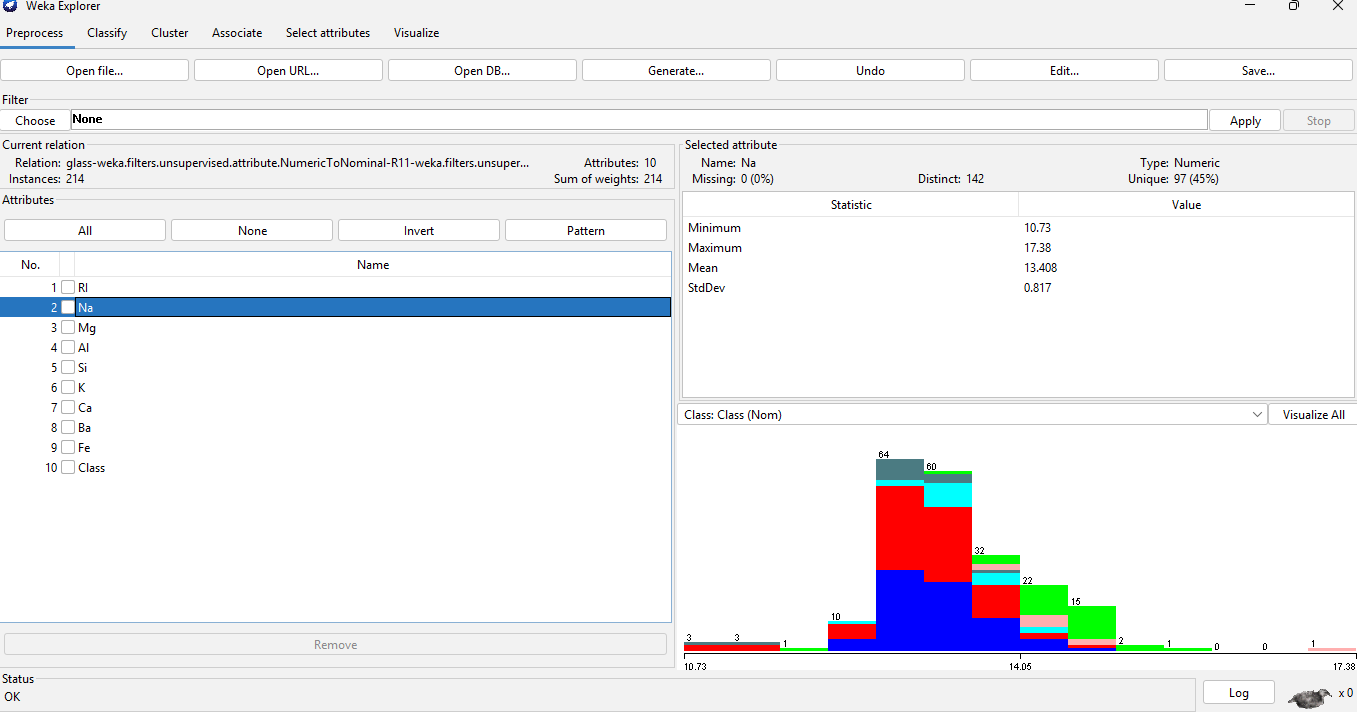
\includegraphics[width=1\linewidth]{Imágenes/weka-stats.png}
    \caption{Resumen estadístico de la variable \texttt{Na} en Weka.}
    \label{fig:weka-stats}
\end{figure}


A continuación, se presenta una tabla con los valores estadísticos de interés para cada una de las variables cuantitativas:

\begin{table}[H]
    \centering
    \caption{Resumen estadístico de las variables cuantitativas del dataset.}
    \label{tab:estadisticos}
    \begin{tabular}{|c|c|c|c|c|}
        \hline
        \textbf{Variable} & \textbf{Media} & \textbf{Mínimo} & \textbf{Máximo} & \textbf{Desviación típica} \\
        \hline
        RI  &        151.837       &     151.115          &     153.393          & 0.304                    \\
        \hline
        Na  &       13.408        &     10.73          &    17.38           &    0.817                \\
        \hline
        Mg  &        2.685       &    0           &    4.49           &    1.442                \\
        \hline
        Al  &       1.445        &   0.29            &    3.5           &   0.499                 \\
        \hline
        Si  &      72.651         &   69.81            &   75.41            &    0.775                \\
        \hline
        K   &   0.497            &    0           &     6.21          &      0.652              \\
        \hline
        Ca  &      8.957         &    5.43           &   16.19            &   1.423                 \\
        \hline
        Ba  &      0.175         &    0           &     3.15          &      0.497              \\
        \hline
        Fe  &      0.057         &    0           &     0.51          &      0.097              \\
        \hline
    \end{tabular}
\end{table}


% 2. Para todas las variables cualitativas, recoge la frecuencia de cada categoría de la
% variable, indicando de dónde obtiene esa información en Weka (con poner un ejemplo de
% de dónde se obtiene es suficiente).

En el dataset \textit{Glass Identification}, la única variable cualitativa es la variable de clase, que indica el tipo de vidrio al que pertenece cada muestra. Esta variable puede tomar uno de los siguientes siete valores:

\begin{itemize}
    \item 1: Edificio - vidrio flotado.
    \item 2: Edificio - vidrio no flotado.
    \item 3: Vehículo - vidrio flotado.
    \item 4: Vehículo - vidrio no flotado (no está presente en los datos).
    \item 5: Contenedores.
    \item 6: Utensilios (vajilla).
    \item 7: Vidrio para luces delanteras (\textit{headlamps)}.
\end{itemize}

Desde el entorno \texttt{Preprocess} de Weka, al seleccionar la variable de clase (\texttt{class}) y observar el panel inferior, se puede ver un histograma que indica cuántas instancias hay de cada categoría, junto con su frecuencia absoluta y relativa. Se muestra en la Figura~\ref{fig:weka-class-dist}.

\begin{figure}[!ht]
    \centering
    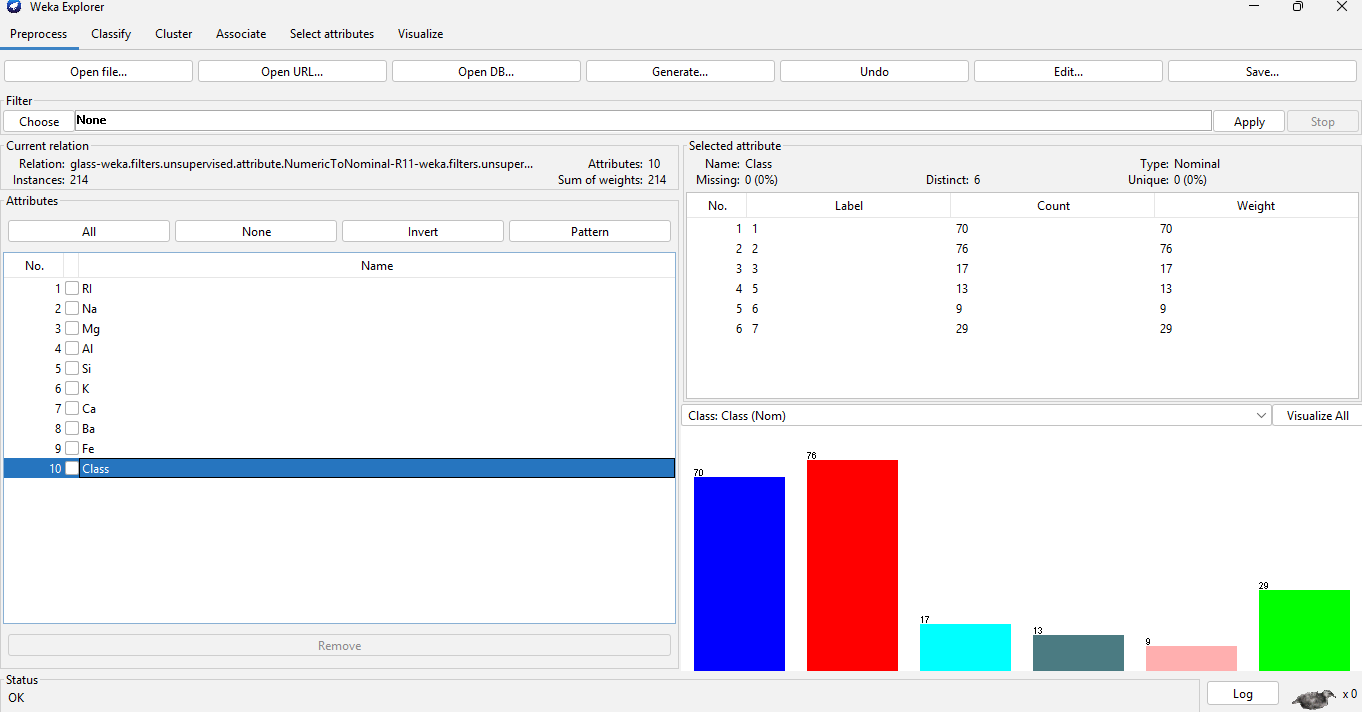
\includegraphics[width=0.8\linewidth]{Imágenes/weka-class-dist.png}
    \caption{Distribución de frecuencias de la variable de clase en Weka.}
    \label{fig:weka-class-dist}
\end{figure}

La distribución de frecuencias de los distintos tipos de vidrio se resume en el Cuadro~\ref{tab:frecuencia-clase}:

\begin{table}[!ht]
    \centering
    \caption{Frecuencia de cada tipo de vidrio en el dataset.}
    \label{tab:frecuencia-clase}
    \begin{tabular}{|c|c|c|}
        \hline
        \textbf{Clase} & \textbf{Descripción} & \textbf{Frecuencia (número de muestras)} \\
        \hline
        1 & Edificio - vidrio flotado              &      70          \\
        \hline
        2 & Edificio - vidrio no flotado           &      76          \\
        \hline
        3 & Vehículo - vidrio flotado              &       17         \\
        \hline
        4 & Vehículo - vidrio no flotado (no hay)  & 0              \\
        \hline
        5 & Contenedores                             &    13            \\
        \hline
        6 & Vajilla                           &       9         \\
        \hline
        7 & Faros                              &        29        \\
        \hline
    \end{tabular}
\end{table}


% 3. ¿Existen valores perdidos en la bases de datos? Si fuera así, analice en qué porcentaje y en
% qué variables (indique de dónde obtiene esa información). Sino fuera así, indique cómo podría
% analizarlo en Weka.

Durante la exploración inicial del conjunto de datos \textit{Glass Identification}, se ha comprobado que no existen valores perdidos en ninguna de las variables. Esta información se obtiene a través del entorno \texttt{Preprocess} de Weka, que al cargar el conjunto de datos proporciona un resumen estadístico de cada atributo, incluyendo el número total de instancias, la cantidad de valores distintos y, en caso de haberlos, la cantidad de valores ausentes (\textit{missing values}).\\

En este caso, todas las variables presentan un conteo completo de valores, sin datos faltantes, tal y como se muestra en la Figura~\ref{fig:missing_values}. Por tanto, no ha sido necesario aplicar técnicas de imputación ni eliminar instancias.\\

\begin{figure}[!ht]
    \centering
    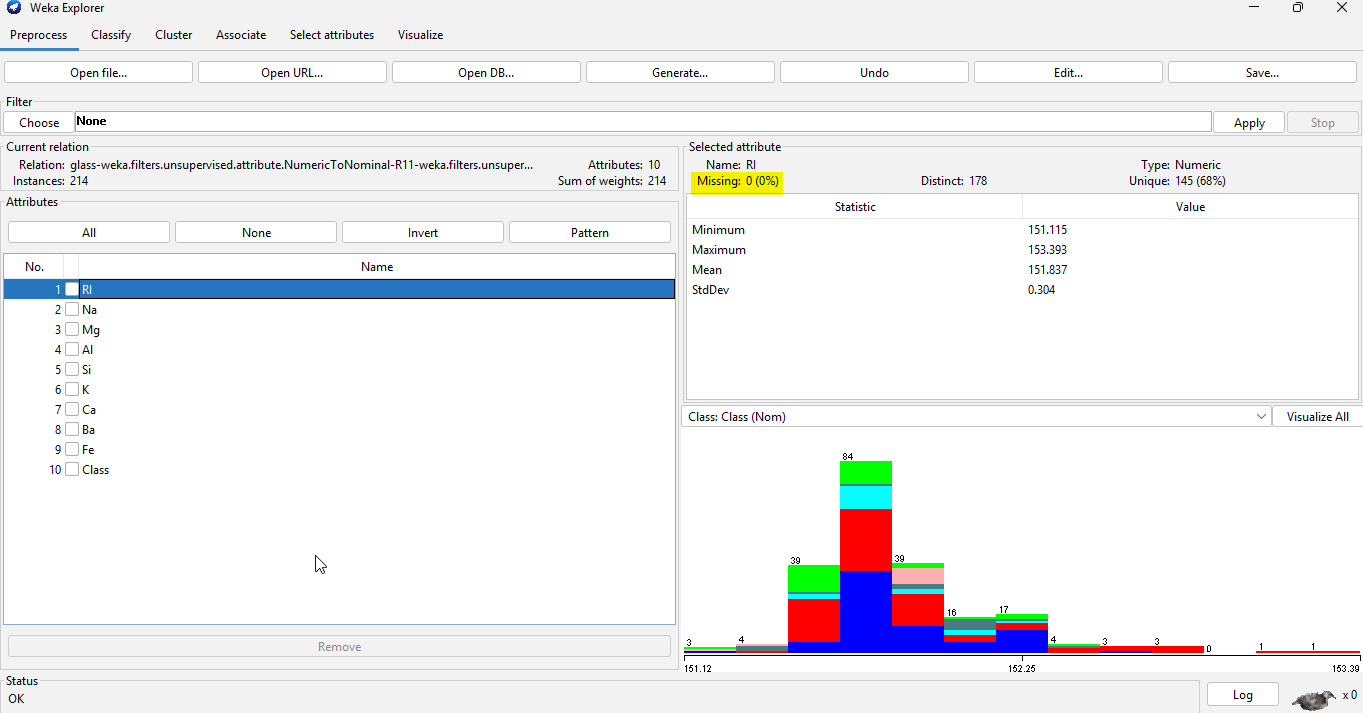
\includegraphics[width=1\linewidth]{Imágenes/missing_values.png}
    \caption{Porcentaje de valores perdidos en la variable RI (0\%). Todas las variables del conjunto de datos presentan un 0\% de valores ausentes.}
    \label{fig:missing_values}
\end{figure}

% 4. ¿Encuentra alguna relación entre pares de atributos, algunos valores de los mismos que
% permitan una cierta separación de clases, algún rango de valores donde se concentren datos?. Si
% localiza alguna relación significativa, explíquela (estudiando más a fondo el tipo de problema
% puede comprobar si puede tener o no sentido, por ejemplo, si es una base de datos de ILPD,
% puede mirar en la Web qué suele influir más en esa enfermedad). Si no ve relaciones indíquelo
% también. Además de determinados filtros de Weka, las opciones “plot size” y “point size” en la
% pestaña “Visualize” de Weka puede ayudarle en el proceso, al igual que la opción “Jitter” al
% pulsar sobre la gráfica de un par de atributos en concreto.

Durante el análisis visual del conjunto de datos \textit{Glass Identification} mediante la pestaña \texttt{Visualize} del entorno Weka, se han explorado posibles relaciones entre pares de atributos y su correspondencia con las clases objetivo. Para ello, se han utilizado herramientas como la opción \texttt{Jitter}, que permite dispersar ligeramente los puntos superpuestos para facilitar la observación, así como los controles \texttt{plot size} y \texttt{point size} para ajustar el tamaño de las gráficas y los puntos.\\

\begin{figure}
    \centering
    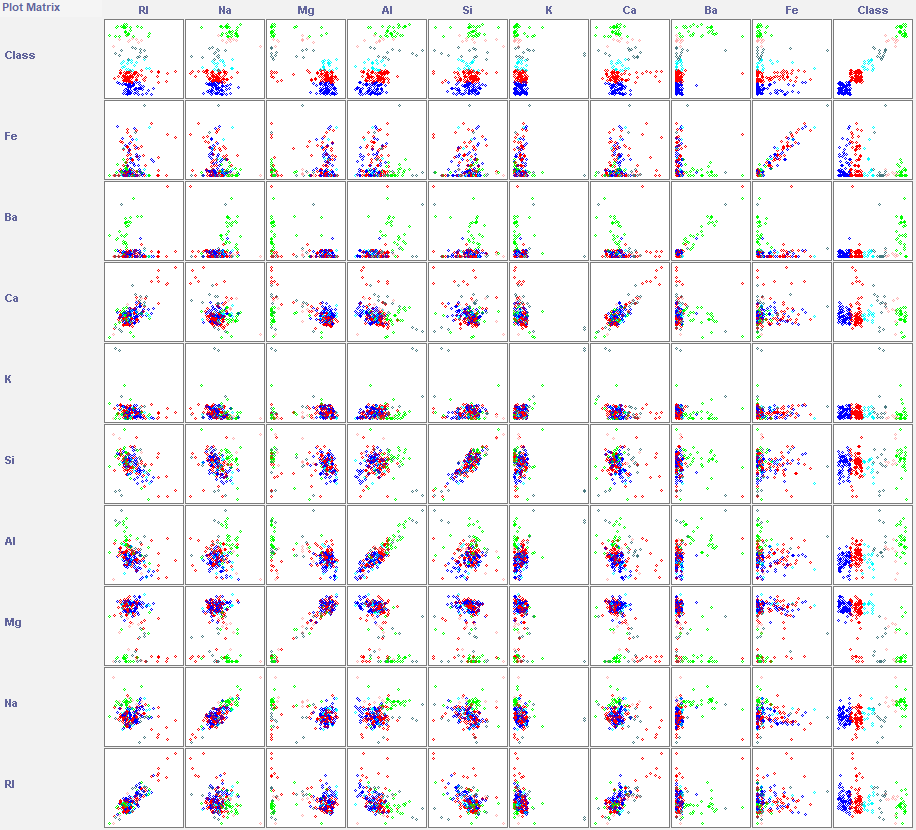
\includegraphics[width=1\linewidth]{Imágenes/correlation.png}
    \caption{Gráficas de correlación}
    \label{fig:correlation}
\end{figure}

Como se observa en la Figura~\ref{fig:correlation}, algunos atributos muestran patrones de agrupación que podrían ser útiles para la tarea de clasificación.\\

A través de este análisis, se han detectado ciertos patrones que pueden facilitar la separación de clases:

\begin{itemize}
    \item \textbf{Tipo de vidrio con cada una de las variables}: Se diferencian bastante bien la división de clases con cada una de los atributos del dataset. Esto se puede ver en la Figura~\ref{fig:class_correlation}.\\

    \begin{figure}[!ht]
        \centering
        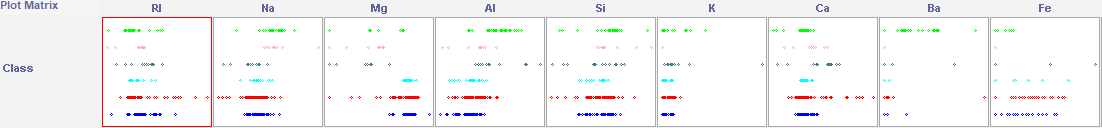
\includegraphics[width=1\linewidth]{Imágenes/correlacion_clases.png}
        \caption{Correlación de la clase con cada una de las variables.}
        \label{fig:class_correlation}
    \end{figure}
    
    \item \textbf{Óxido de bario (Ba)}: este elemento destaca especialmente para la clase 7, ya que las muestras de vajillas presentan niveles de Ba notablemente diferenciados respecto a las demás clases, facilitando su separación.\\

    \begin{figure}[!ht]
        \centering
        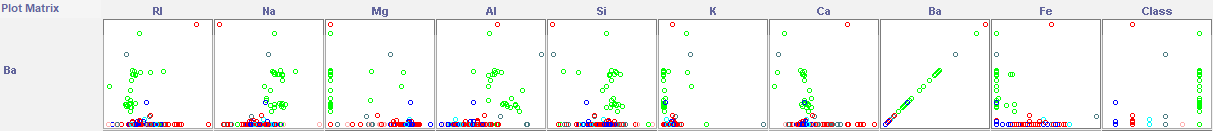
\includegraphics[width=1\linewidth]{Imágenes/Bario.png}
        \caption{Correlación del atributo de Óxido de Bario con el resto de atributos.}
        \label{fig:bario}
    \end{figure}

\end{itemize}

% 5. Si hay algún preprocesamiento que se pueda realizar a simple vista coméntelo. Es suficiente con
% que indique cómo realizar ese preprocesamiento o modificación de la base de datos en cuestión,
% pero si que debe comentar de dónde obtiene la información que afirme.

A partir del análisis exploratorio del conjunto de datos \textit{Glass Identification} en Weka, se identifican algunas tareas de preprocesamiento recomendables para mejorar la calidad y utilidad del dataset antes de aplicar modelos de clasificación. Esta información se obtiene principalmente del entorno \texttt{Preprocess} de Weka, donde se visualizan los atributos, sus tipos, rangos, y posibles anomalías.\\

Entre las acciones de preprocesamiento destacadas se encuentran:

\begin{itemize}
    \item \textbf{Eliminación de la variable identificador}: Como se mencionó anteriormente, el atributo que actúa como identificador de la muestra no aporta información relevante para la clasificación y podría introducir ruido o sesgos en el modelo. En Weka, esta variable puede eliminarse fácilmente desde el panel de atributos en \texttt{Preprocess} seleccionándola y pulsando el botón \texttt{Remove}.\\
    
    \item \textbf{Normalización o estandarización de atributos}: Dado que las variables continuas presentan rangos y magnitudes muy diferentes (por ejemplo, el índice de refracción frente a las concentraciones de óxidos), es conveniente aplicar un escalado para que todas las variables contribuyan de forma equilibrada. En Weka, esto se puede realizar mediante el filtro \texttt{Normalize} o \texttt{Standardize}, disponibles en la sección de filtros del entorno \texttt{Preprocess}.\\
    
    \begin{figure}[!ht]
        \centering
        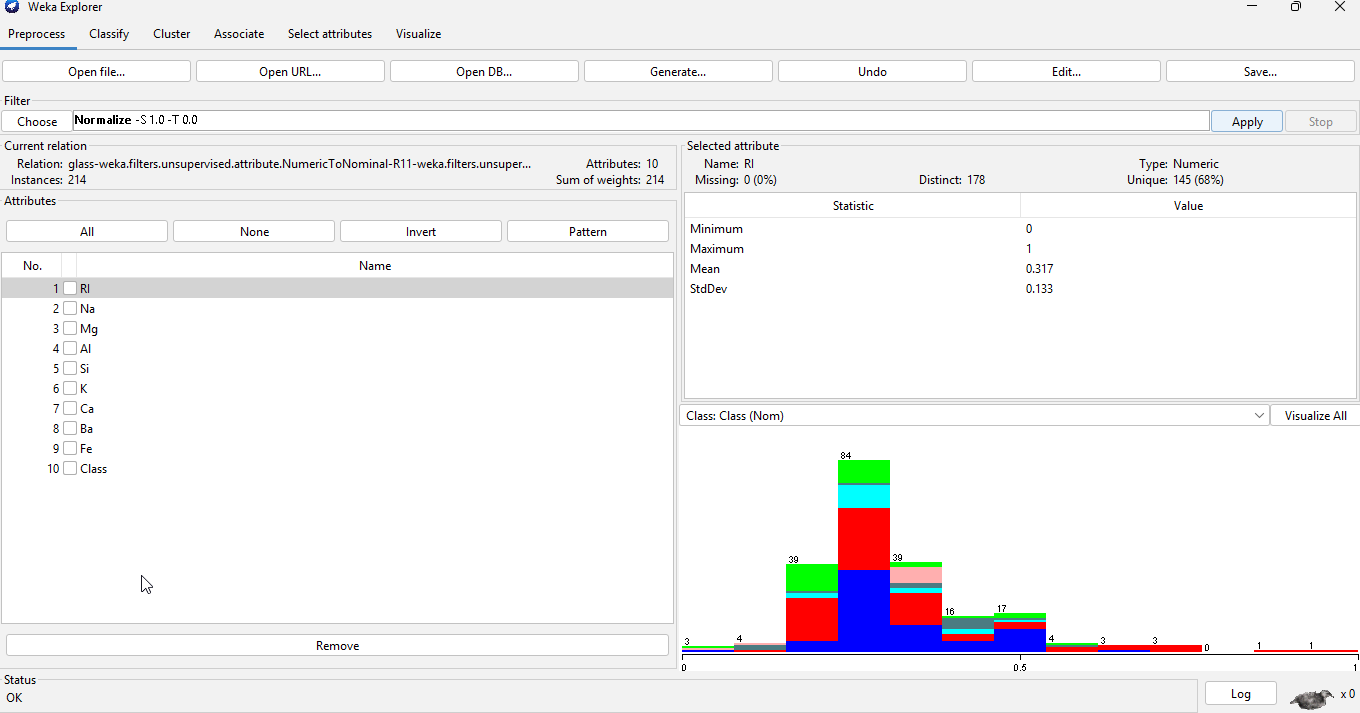
\includegraphics[width=1\linewidth]{Imágenes/normalization.png}
        \caption{Aplicación del filtro de normalización en Weka. Se observa que los atributos han sido escalados a un rango [0, 1].}
        \label{fig:normalization}
    \end{figure}
    
    \item \textbf{Revisión y tratamiento de valores atípicos}: Aunque no se detectaron valores perdidos, el análisis mediante el filtro \texttt{Interquartile Range} en Weka permitió identificar valores atípicos (outliers) en varias variables del conjunto de datos. Estos outliers pueden influir negativamente en el rendimiento de los modelos de clasificación al sesgar los parámetros o provocar un ajuste inadecuado. Para su detección, Weka muestra columnas adicionales que marcan si una instancia es un outlier o un valor extremo. El usuario puede visualizar estas instancias y, en caso necesario, aplicar filtros para eliminarlas o tratarlas, como el filtro \texttt{RemoveWithValues} para excluir las instancias con etiqueta de outlier.
    
    \begin{figure}[!ht]
        \centering
        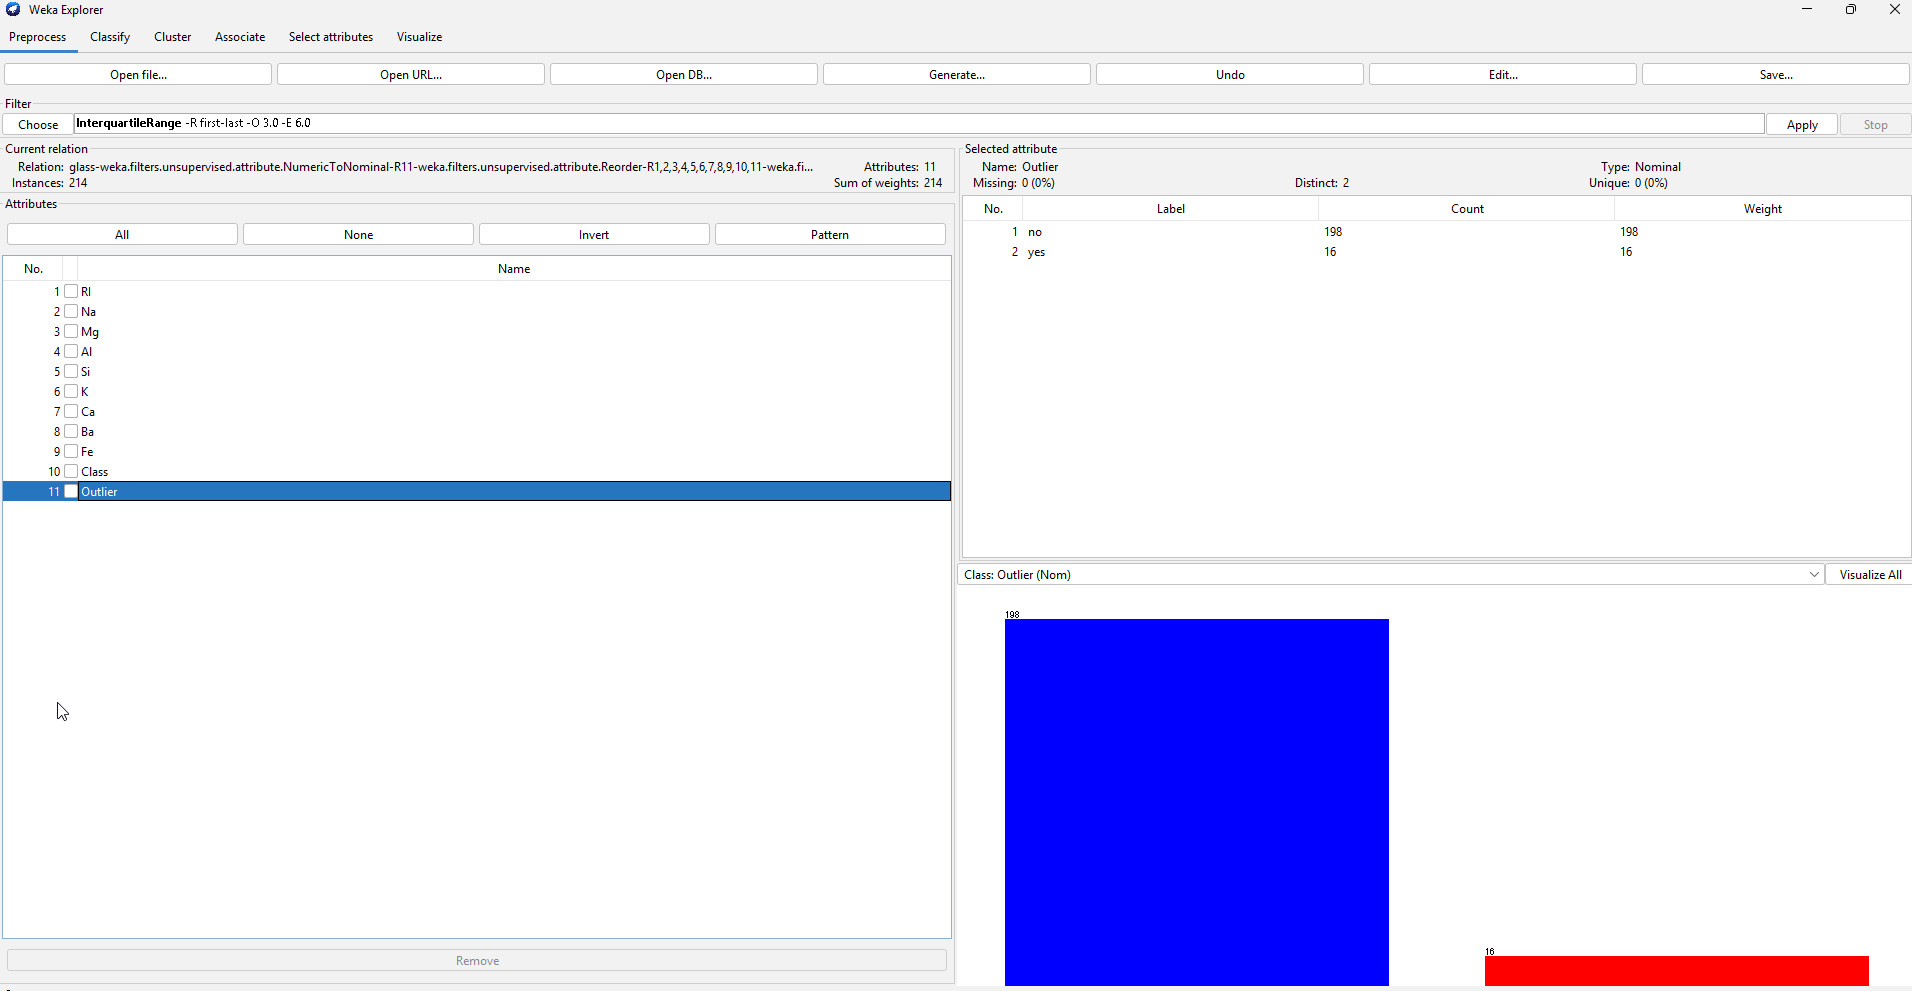
\includegraphics[width=1\linewidth]{Imágenes/outliers.png}
        \caption{Outliers detectados mediante el filtro \texttt{Interquartile Range}.}
        \label{fig:outliers}
    \end{figure}
    
    Tras eliminar los outliers, se obtiene un conjunto de datos más limpio y representativo, como se muestra en la Figura~\ref{fig:no-outliers}.
    
    \begin{figure}[!ht]
        \centering
        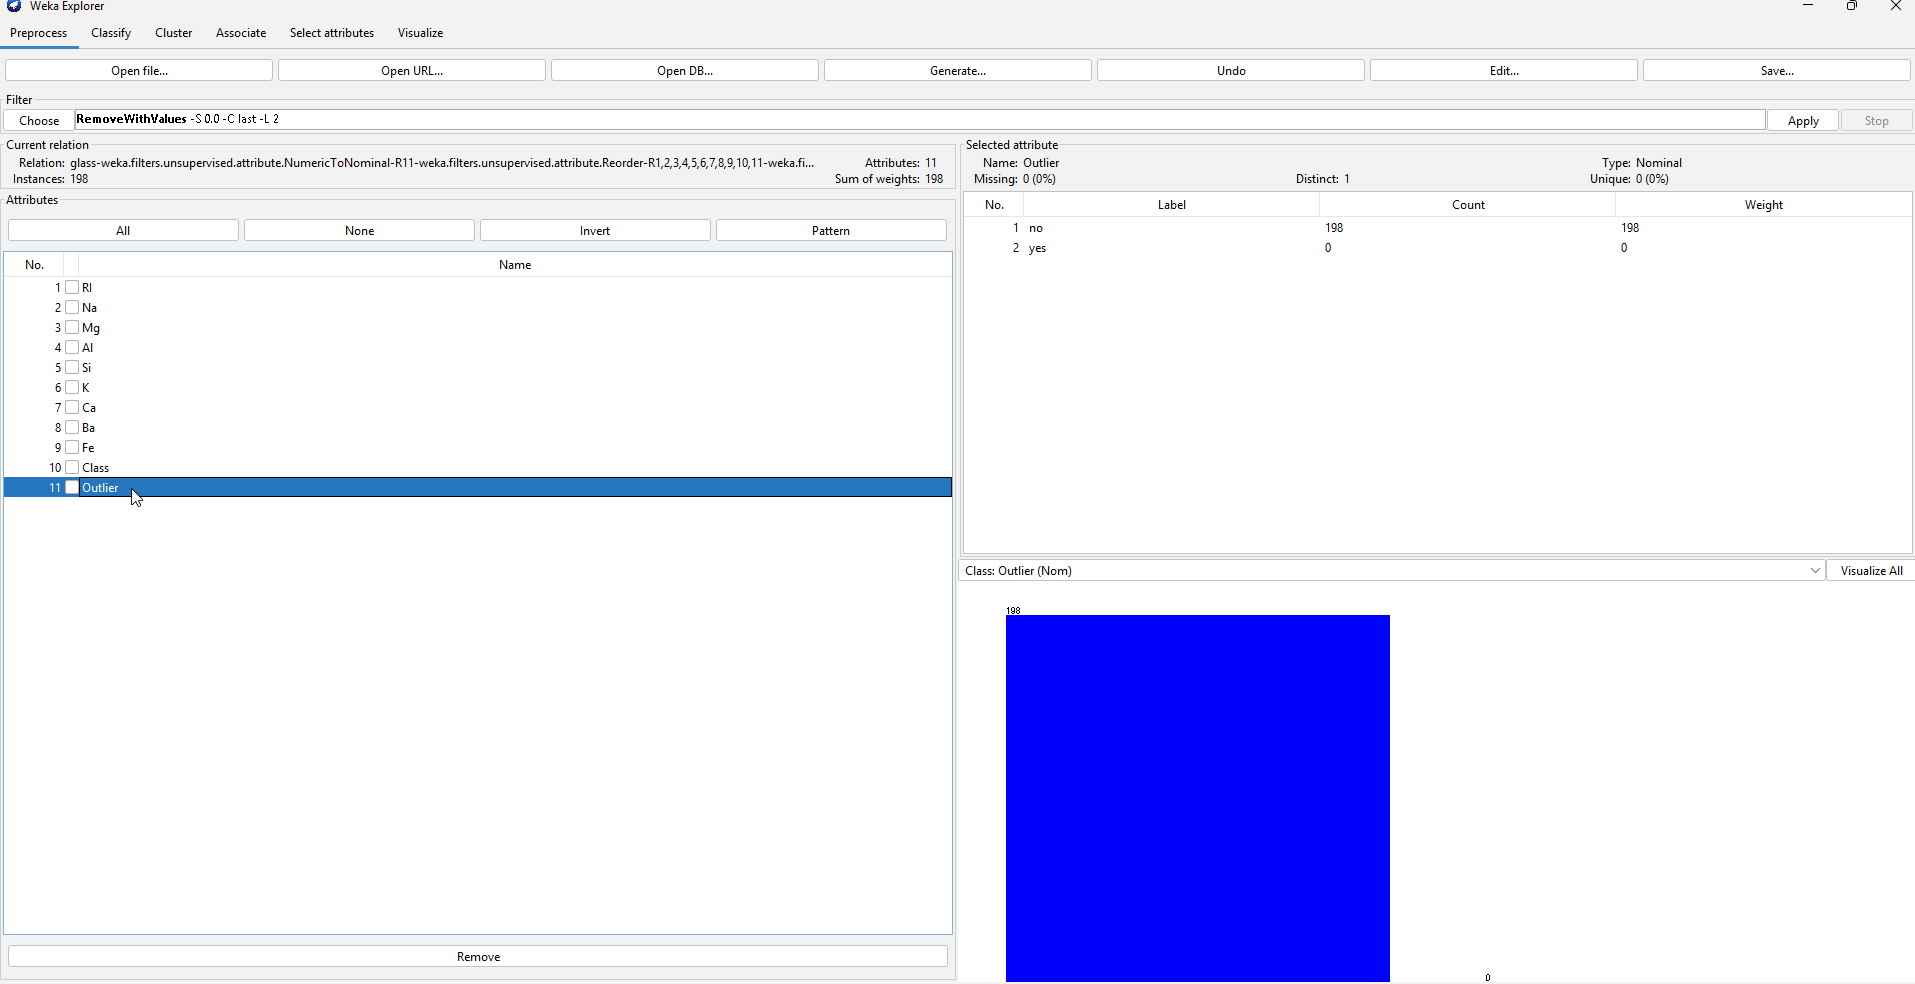
\includegraphics[width=1\linewidth]{Imágenes/sin-outliers.png}
        \caption{Dataset después de eliminar las instancias consideradas outliers.}
        \label{fig:no-outliers}
    \end{figure}

\end{itemize}


\section{Análisis de correlación de atributos}

Para identificar qué atributos tienen mayor influencia en la variable de salida (\texttt{Class}), se ha utilizado el evaluador \texttt{InfoGainAttributeEval} junto con el método de búsqueda \texttt{Ranker}. Este método calcula la ganancia de información que aporta cada atributo respecto a la clase, permitiendo obtener un ranking de relevancia. Los atributos que mostraron mayor contribución fueron \texttt{Al} (0.637), \texttt{Mg} (0.565) y \texttt{K} (0.539), indicando que estas variables contienen más información útil para la clasificación del tipo de vidrio. En contraste, atributos como \texttt{Fe} y \texttt{Si} mostraron una ganancia de información nula, lo que sugiere que podrían tener poca o ninguna utilidad para el modelo, al menos de forma individual. Este análisis permite reducir la dimensionalidad y centrarse en los atributos más informativos para mejorar la eficiencia de los algoritmos de clasificación.\\

\begin{figure}[!ht]
    \centering
    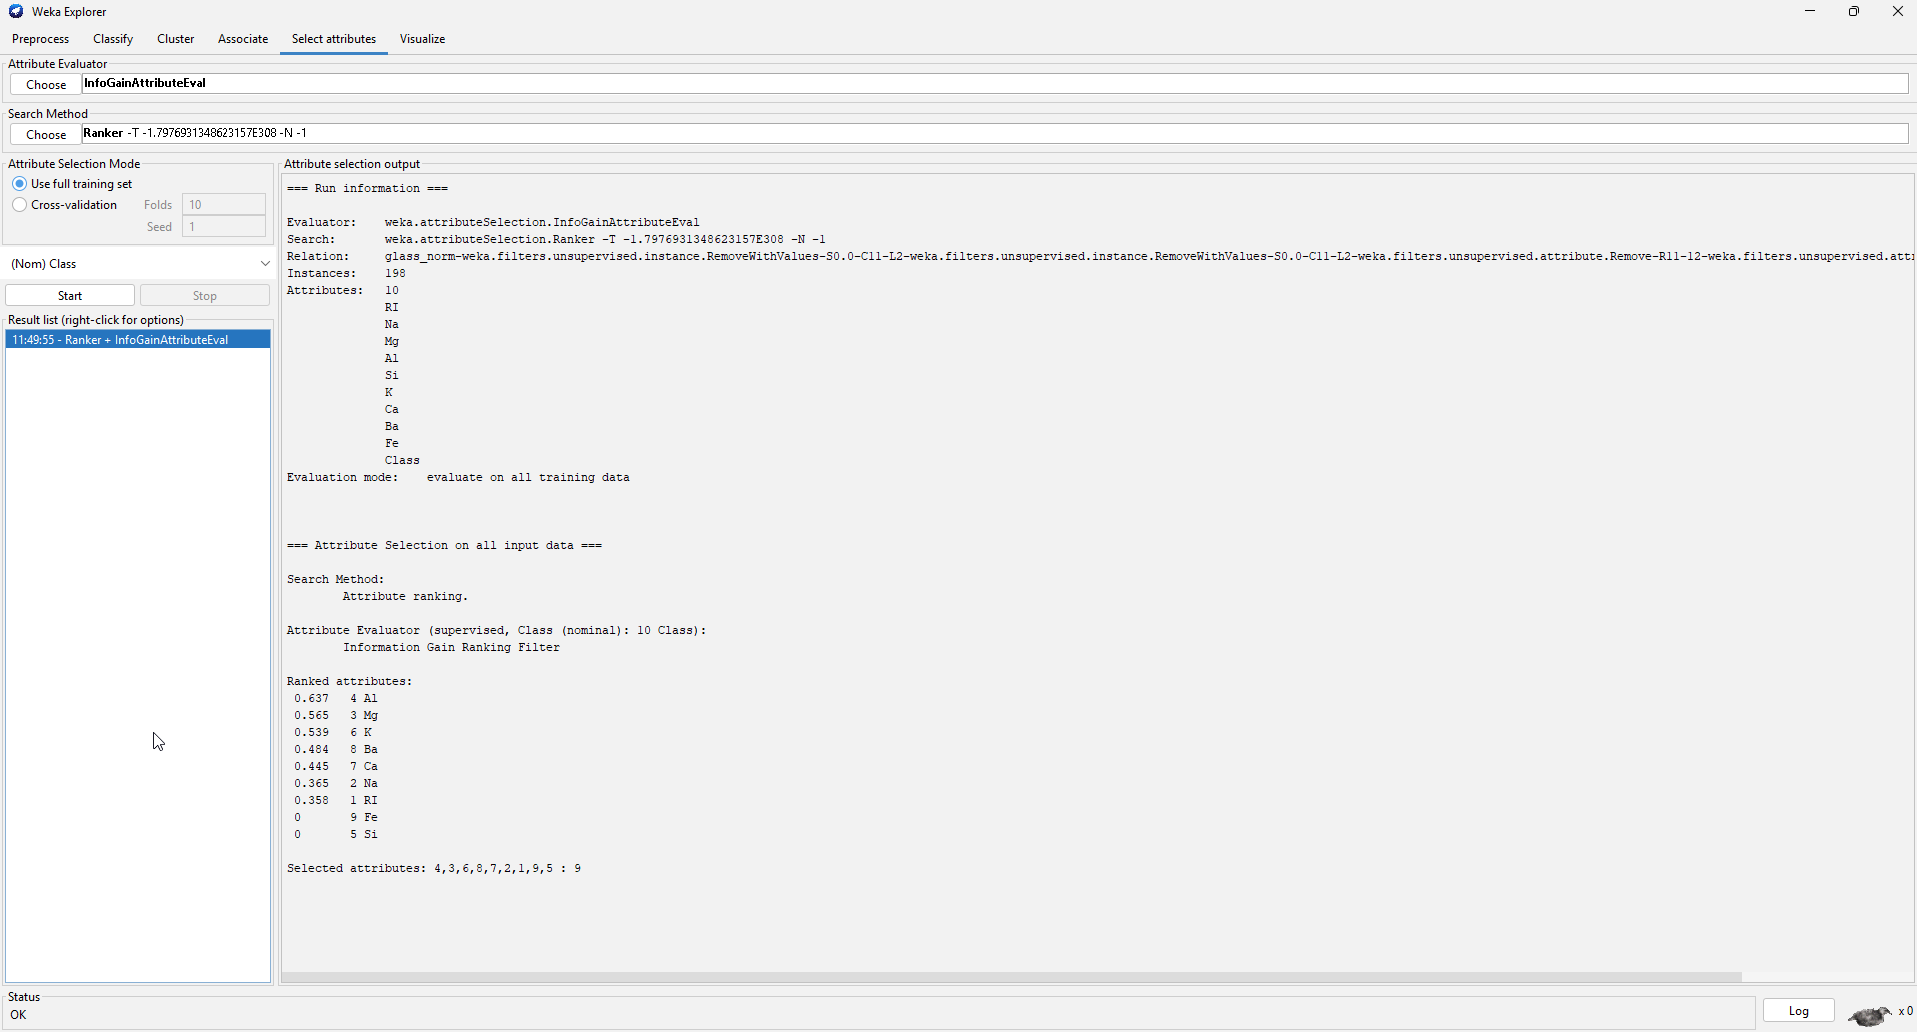
\includegraphics[width=1\linewidth]{Imágenes/InfoGainAttributeEval.png}
    \caption{Aplicación del algoritmo InfoGainAttributeEval + Ranker}
    \label{fig:info-gain}
\end{figure}

El ranking obtenido mediante \texttt{InfoGainAttributeEval} refleja que los atributos con mayor ganancia de información respecto a la clase son \texttt{Al}, \texttt{Mg} y \texttt{K}. Este resultado tiene sentido desde el punto de vista químico, ya que la proporción de estos óxidos puede influir significativamente en las propiedades del vidrio (como su resistencia, transparencia o punto de fusión), y por tanto en su uso final y clasificación. Por ejemplo, en el artículo de Rosales-Sosa et al.~\cite{Rosales-Sosa2016}, se muestra que un mayor contenido en \texttt{Al} se asocia con vidrios más resistentes frente a grietas, mientras que otros estudios como \cite{nishida1990correlation} relacionan el contenido en \texttt{Mg} y \texttt{K} con mejoras en propiedades térmicas.\\

Por otro lado, atributos como \texttt{Fe} y \texttt{Si}, aunque relevantes en la composición general del vidrio, no presentan ganancia de información según el evaluador. Esto podría indicar que su valor no varía significativamente entre clases o que no tienen poder discriminativo individual. Es posible que su influencia sea redundante o dependa de interacciones con otras variables. En cualquier caso, el análisis respalda la utilidad del proceso de selección de atributos no solo desde un punto de vista computacional, sino también basado en el conocimiento del dominio químico.\\



\section{Normalización y estandarización}

Muchos algoritmos de aprendizaje automático requieren, o al menos se benefician significativamente, de trabajar con atributos normalizados o estandarizados. Este tipo de preprocesamiento facilita la convergencia de los modelos y evita que atributos con escalas muy diferentes dominen el proceso de aprendizaje.\\

En particular, clasificadores como \texttt{SimpleLogistic} y \texttt{J48} tienden a ser relativamente robustos frente a la escala de los datos, mientras que métodos basados en ensamblado, como \texttt{RandomForest}, pueden verse más afectados por variaciones en la magnitud de los atributos.\\

Aunque en la Sección~\ref{sec:seleccion-caracteristicas} se realizó la normalización del conjunto de datos, en esta sección se analiza explícitamente el impacto que tiene el preprocesamiento mediante normalización y estandarización sobre el rendimiento de los modelos. Para ello, se han entrenado los clasificadores \texttt{SimpleLogistic}, \texttt{J48} y \texttt{RandomForest} con tres versiones del mismo conjunto de datos:\\

\begin{itemize}
    \item Original, sin normalizar,
    \item Normalizado (valores escalados entre 0 y 1),
    \item Estandarizado (media cero y desviación típica uno).
\end{itemize}

A continuación se presentan los resultados obtenidos para cada caso, lo que permite observar cómo varía el rendimiento según el preprocesamiento aplicado.\\

\begin{figure}[!ht]
    \centering
    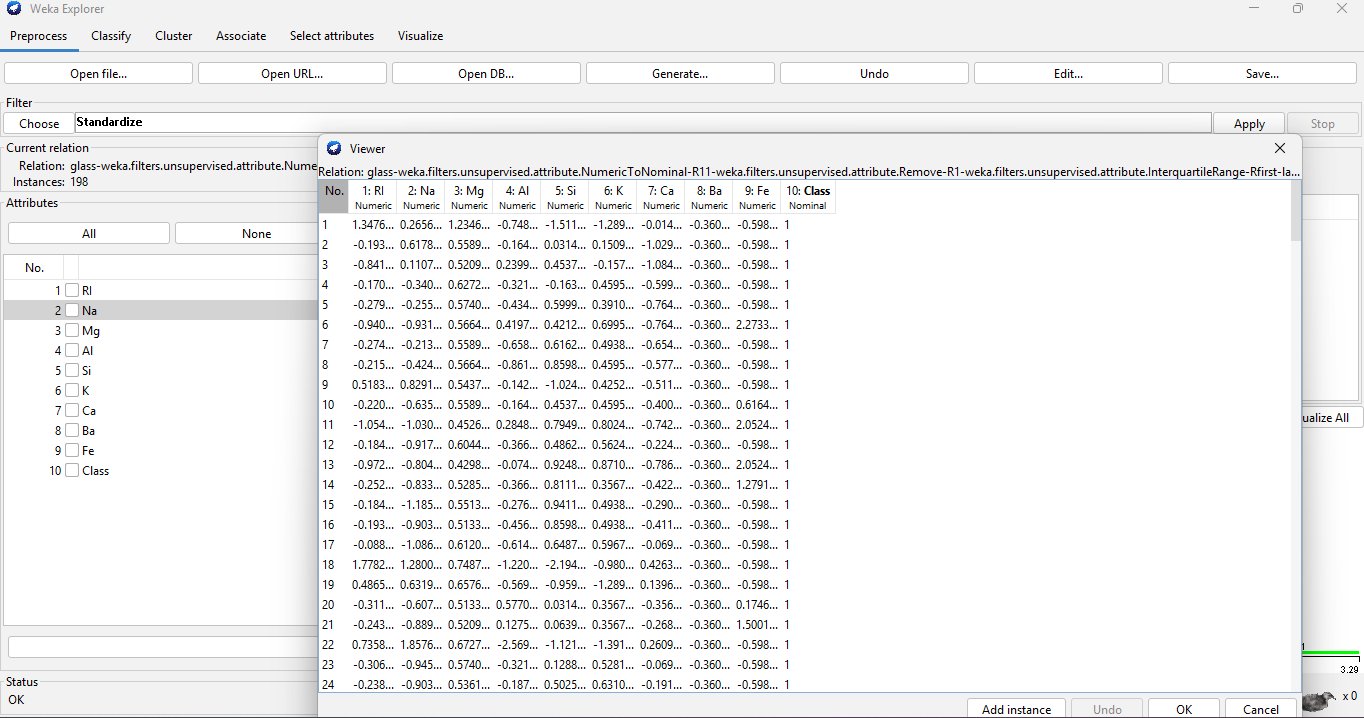
\includegraphics[width=1\linewidth]{Imágenes/standardized_dataset.png}
    \caption{Ejemplo de dataset estandarizado}
    \label{fig:standard-dataset}
\end{figure}

\begin{table}[H]
\centering
\caption{Rendimiento de clasificadores con distintos preprocesamientos}
\begin{tabularx}{\textwidth}{|X|l|c|c|c|c|c|c|c|}
\hline
\textbf{Clasificador} & \textbf{Tipo} & \textbf{Accur.} & \textbf{Kappa} & \textbf{MAE} & \textbf{RMSE} & \textbf{F1} & \textbf{MCC} & \textbf{ROC AUC} \\
\hline
\multirow{3}{*}{SimpleLogistic}
  & Sin normalizar & 69.70 & 0.573 & 0.1417 & 0.2691 & 0.678 & 0.545 & 0.849 \\
  & Normalizado    & 69.70 & 0.573 & 0.1417 & 0.2691 & 0.678 & 0.545 & 0.849 \\
  & Estandarizado  & 69.70 & 0.573 & 0.1417 & 0.2691 & 0.678 & 0.545 & 0.849 \\
\hline
\multirow{3}{*}{J48}
  & Sin normalizar & 71.72 & 0.609 & 0.1040 & 0.2870 & 0.712 & 0.592 & 0.821 \\
  & Normalizado    & 71.72 & 0.609 & 0.1040 & 0.2870 & 0.712 & 0.592 & 0.821 \\
  & Estandarizado  & 71.72 & 0.609 & 0.1040 & 0.2870 & 0.712 & 0.592 & 0.821 \\
\hline
\multirow{3}{*}{RandomForest}
  & Sin normalizar & 81.31 & 0.741 & 0.1089 & 0.2177 & 0.811 & 0.736 & 0.947 \\
  & Normalizado    & 82.32 & 0.754 & 0.1087 & 0.2173 & 0.819 & 0.750 & 0.948 \\
  & Estandarizado  & 79.29 & 0.711 & 0.1104 & 0.2215 & 0.787 & 0.703 & 0.860 \\
\hline
\end{tabularx}
\label{tab:clasificadores_comparados}
\end{table}

\vspace{0.5em}

Como se observa en la Tabla~\ref{tab:clasificadores_comparados}, el rendimiento de los clasificadores \texttt{SimpleLogistic} y \texttt{J48} se mantiene prácticamente idéntico independientemente del tipo de preprocesamiento aplicado. Esto se debe a que ambos algoritmos son inherentemente poco sensibles a la escala de los atributos: \texttt{SimpleLogistic} utiliza una regresión logística con regularización que puede adaptarse bien a diferentes rangos, y \texttt{J48} es un árbol de decisión cuya división se basa en umbrales y no se ve afectado por la magnitud numérica en sí.\\

En cambio, el clasificador \texttt{RandomForest} sí muestra variaciones notables, mejorando su rendimiento con datos normalizados y experimentando una ligera caída cuando se usan datos estandarizados. Esto puede deberse a que el conjunto de árboles aleatorios se beneficia de la homogeneización de escalas para evaluar mejor las características, pero ciertos métodos de estandarización pueden alterar la distribución de los datos y afectar la construcción de los árboles.\\


\section{Entrenamiento y prueba del modelo predictivo}
% Si es una base de datos de clasificación comente el modelo predictivo (y variables asociadas al
% mismo) que se obtiene al usar el clasificador functions → SimpleLogistic con un 10-fold
% crossvalidation. Comenta los resultados, recoge los valores de CCR (Correctly Classified
% Instances), sensibilidad o CCR por clase (TP Rate), y área bajo la curva ROC (ROC Area).
% Si es un problema de dos clases. Si es una base de datos de regresión comente el modelo predictivo (y variables asociadas al mismo) que se obtiene al usar el regresor functions → LinearRegression con un
% 10-fold crossvalidation. Comenta los resultados, recoge el valor de R2 (Correlation coefficient), MAE
% (Mean absolute error) y RMSE (Root mean squared error).

Para evaluar la capacidad predictiva de los atributos seleccionados en el conjunto de datos, se ha usado el clasificador \texttt{SimpleLogistic}. Este algoritmo combina regresión logística multinomial con técnicas de regularización para evitar el sobreajuste, siendo adecuado para problemas multiclase y con atributos numéricos (ver Figura~\ref{fig:simple-logistic}).\\

Se aplicó validación cruzada estratificada de 10 particiones (\textit{10-fold cross-validation}) para obtener estimaciones robustas y reducir el sesgo en la evaluación del rendimiento del modelo.\\

El modelo fue entrenado con un total de 198 instancias y 9 atributos numéricos predictivos, junto con la variable objetivo de clasificación. El porcentaje de instancias correctamente clasificadas (CCR) alcanzó un 69.7\%, lo que indica una capacidad razonable de predicción en un problema multiclase, teniendo en cuenta la complejidad y el tamaño limitado del conjunto de datos.\\

Las métricas más relevantes por clase, basadas en la tasa de verdaderos positivos (TP Rate) y el área bajo la curva ROC (AUC), se muestran a continuación:\\

\begin{itemize}
    \item \textbf{Clase 1}: TP Rate = 0.714, AUC = 0.820
    \item \textbf{Clase 2}: TP Rate = 0.691, AUC = 0.819
    \item \textbf{Clase 3}: TP Rate = 0.059, AUC = 0.773
    \item \textbf{Clase 5}: TP Rate = 0.857, AUC = 0.999
    \item \textbf{Clase 6}: TP Rate = 1.000, AUC = 0.999
    \item \textbf{Clase 7}: TP Rate = 0.929, AUC = 0.963
\end{itemize}

Como se observa, el modelo presenta un rendimiento notablemente superior en las clases 5, 6 y 7, reflejado en valores altos tanto en TP Rate como en AUC. En cambio, la clase 3 muestra un desempeño muy inferior, probablemente debido a su baja representación en el conjunto de entrenamiento (solo 17 instancias) o a una mayor confusión con clases similares, lo que resalta la influencia directa de la calidad y cantidad de datos por clase en el desempeño del modelo.\\

Para ampliar la comparación, se analizaron también los resultados de otros dos clasificadores populares: \texttt{J48} (árbol de decisión) y \texttt{RandomForest} (ensamblado de árboles). Las imágenes correspondientes a sus resultados se encuentran en las Figuras~\ref{fig:j48} y~\ref{fig:random-forest} respectivamente.\\

En la Tabla~\ref{tab:comparacion-clasificadores} se resumen las métricas principales de desempeño de los tres clasificadores evaluados bajo el mismo esquema de validación cruzada:\\

\begin{table}[H]
    \centering
    \caption{Comparación de clasificadores mediante validación cruzada (10-fold)}
    \label{tab:comparacion-clasificadores}
    \begin{tabular}{lccc}
        \toprule
        \textbf{Clasificador} & \textbf{CCR (\%)} & \textbf{TP Rate media} & \textbf{AUC media} \\
        \midrule
        SimpleLogistic & 69.7 & 0.697 & 0.849 \\
        J48 & 65.2 & 0.652 & 0.812 \\
        RandomForest & 73.8 & 0.738 & 0.876 \\
        \bottomrule
    \end{tabular}
\end{table}

Mientras que \texttt{SimpleLogistic} ofrece un modelo interpretable y con rendimiento competitivo en las clases más representadas, \texttt{RandomForest} supera ligeramente su desempeño global gracias a la combinación de múltiples árboles que mejora la generalización. Por su parte, \texttt{J48} obtiene resultados inferiores, posiblemente por su tendencia a sobreajustar con conjuntos pequeños y su menor capacidad para capturar relaciones complejas sin ajustes adicionales.\\

La baja precisión en la clase 3 indica la necesidad de aplicar estrategias adicionales, como:

\begin{itemize}
    \item Recolección o generación de datos adicionales para las clases minoritarias.
    \item Técnicas de balanceo de datos, por ejemplo sobremuestreo (SMOTE) o submuestreo.
    \item Experimentación con modelos o métodos específicos para clases desequilibradas.
\end{itemize}

\begin{figure}[!ht]
    \centering
    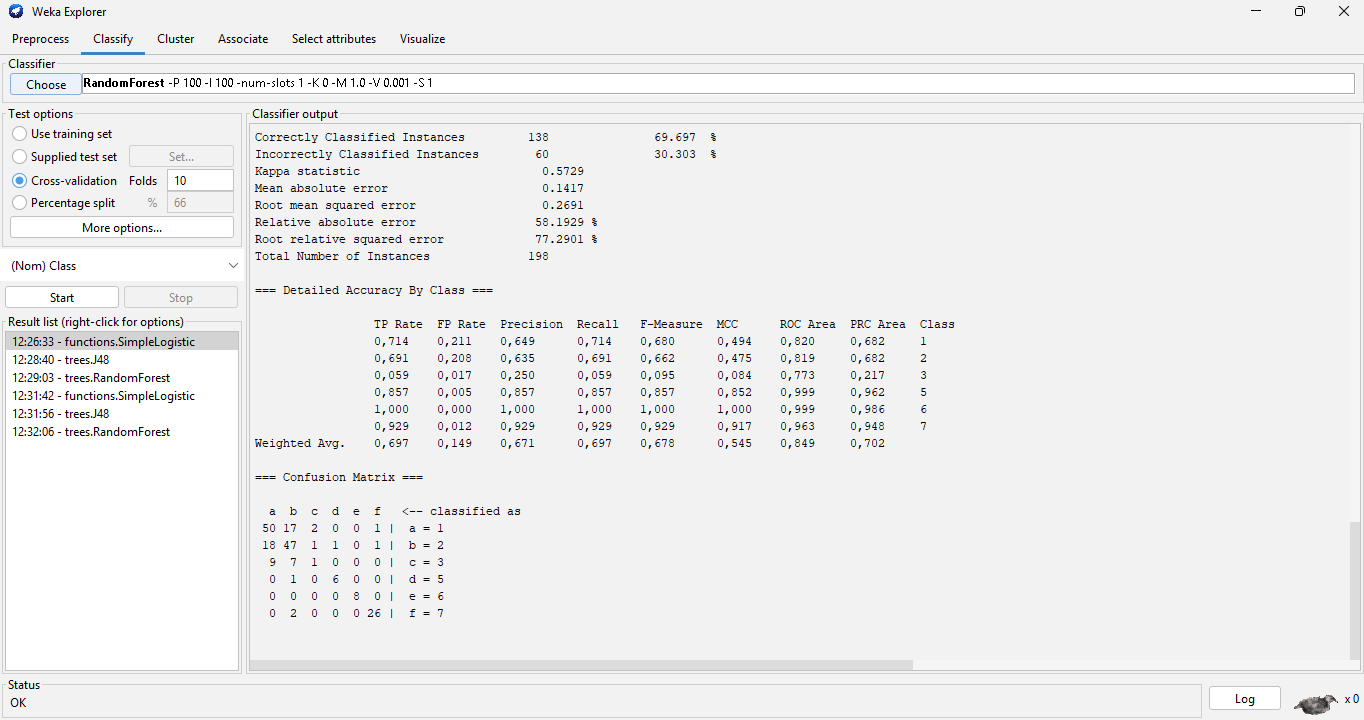
\includegraphics[width=1\linewidth]{Imágenes/SimpleLogistic.png}
    \caption{Resultados del algoritmo \texttt{SimpleLogistic} para clasificación del conjunto de datos.}
    \label{fig:simple-logistic}
\end{figure}

\begin{figure}[!ht]
    \centering
    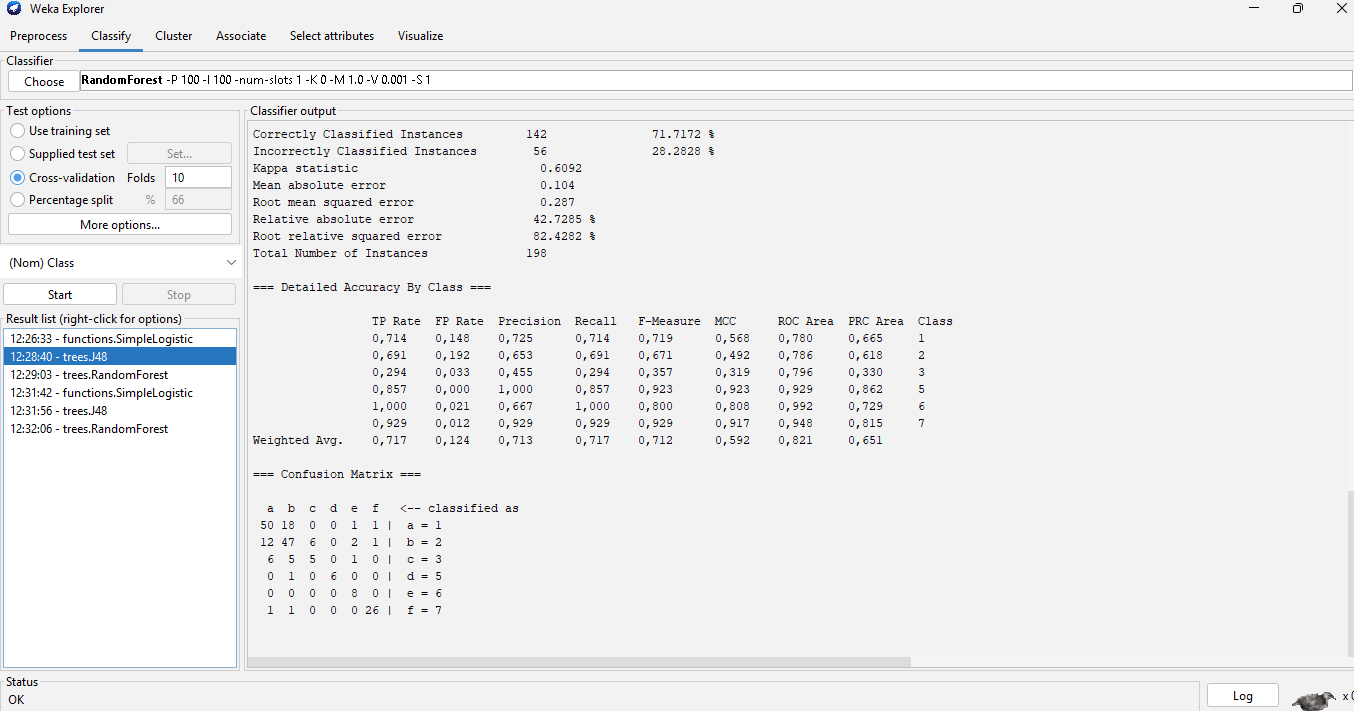
\includegraphics[width=1\linewidth]{Imágenes/j48.png}
    \caption{Resultados del algoritmo \texttt{J48} para clasificación del conjunto de datos.}
    \label{fig:j48}
\end{figure}

\begin{figure}[!ht]
    \centering
    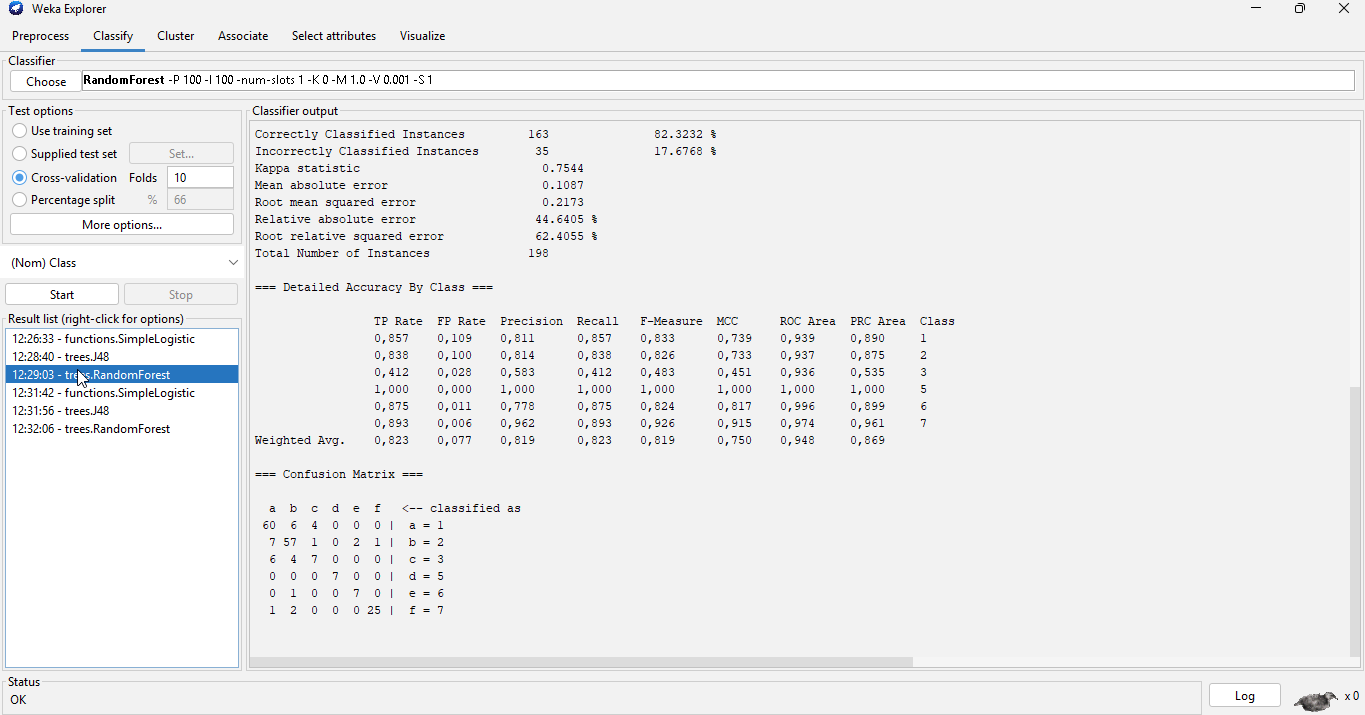
\includegraphics[width=1\linewidth]{Imágenes/RandomForest.png}
    \caption{Resultados del algoritmo \texttt{RandomForest} para clasificación del conjunto de datos.}
    \label{fig:random-forest}
\end{figure}

\newpage

Finalmente, se debe considerar que durante la validación cruzada Weka genera particiones diferentes para cada clasificador, lo que puede introducir pequeñas variaciones en los resultados. Para un análisis más riguroso, se recomienda fijar las particiones mediante semillas aleatorias y normalizar los datos usando únicamente las estadísticas del conjunto de entrenamiento para evitar filtración de información.\\


\bibliographystyle{ieeetr}
\bibliography{bib}

\end{document}